\documentclass[journal]{IEEEtran}

% ---- packages -----------------------------------------------------------
\usepackage[T1]{fontenc}
\usepackage[utf8]{inputenc}
\usepackage{amsmath,amssymb,amsfonts}
\usepackage{algorithmic}
\usepackage{algorithm}
\usepackage{graphicx}
\usepackage{booktabs}
\usepackage{array}
\usepackage{xcolor}
\usepackage{tikz}
\usepackage{pgfplots}
\pgfplotsset{compat=1.18}
\usepgfplotslibrary{fillbetween}
\usetikzlibrary{arrows.meta,positioning,fit,backgrounds,calc,decorations.pathmorphing,shapes.geometric}
\usepackage{url}
\usepackage[hidelinks]{hyperref}
\usepackage{cite}

% ---- palette (navy / steel / amber) -------------------------------------
\definecolor{navy}{RGB}{20,40,90}
\definecolor{steel}{RGB}{70,110,160}
\definecolor{amber}{RGB}{220,150,30}
\definecolor{ink}{RGB}{35,35,40}
\definecolor{paleblue}{RGB}{225,233,245}
\definecolor{palegold}{RGB}{250,238,210}

% ---- shared tikz styles (avoid reserved names) --------------------------
\tikzset{
  box/.style   = {rounded corners=2pt, draw=navy, fill=paleblue, text=ink,
                  align=center, inner sep=4pt, font=\footnotesize},
  hot/.style   = {rounded corners=2pt, draw=amber!80!black, fill=palegold,
                  text=ink, align=center, inner sep=4pt, font=\footnotesize},
  plain/.style = {draw=steel, fill=white, text=ink, align=center,
                  inner sep=3pt, font=\scriptsize},
  flow/.style  = {-{Stealth[length=2.5mm]}, draw=steel, thick},
}

% ---- math shortcuts -----------------------------------------------------
\newcommand{\Lap}{\mathbf{L}}
\newcommand{\Adj}{\mathbf{A}}
\newcommand{\Id}{\mathbf{I}}
\newcommand{\Deg}{\mathbf{D}}
\newcommand{\Eig}{\mathbf{U}}
\newcommand{\Feat}{\mathbf{H}}
\newcommand{\Wt}{\mathbf{W}}
\newcommand{\Prop}{\boldsymbol{\Phi}}
\newcommand{\real}{\mathrm{Re}}
\newcommand{\imag}{\mathrm{Im}}
\DeclareMathOperator{\Var}{Var}

% ---- result numbers (single source of truth; updated from result CSVs) ---
% Result macros -- single source of truth, kept in sync with results/*.csv.
% All values verified against the regenerated canonical CSVs (server run, full
% config: mini264, 5 seeds for B/B2, 8 seeds for C2; commit on 2026-06-26).

% Exp B: operator comparison, mini264 (5 seeds)
\newcommand{\bMAEgcn}{0.163}
\newcommand{\bSTDgcn}{0.016}
\newcommand{\bMAEheat}{0.069}
\newcommand{\bSTDheat}{0.005}
\newcommand{\bMAEqw}{0.071}
\newcommand{\bSTDqw}{0.009}
\newcommand{\bAURCgcn}{0.202}
\newcommand{\bAURCheat}{0.085}
\newcommand{\bAURCqw}{0.077}
\newcommand{\globalgain}{2.3}      % global vs local MAE ratio (0.163/0.069=2.36, /0.071=2.30)

% Exp C1: normalization pitfall (gap-vs-diameter slope), verified vs CSV
\newcommand{\cRawSlope}{0.061}
\newcommand{\cRawMax}{0.63}
\newcommand{\cSFSlope}{0.007}
\newcommand{\cSFMax}{0.05}
\newcommand{\cSlopeRatio}{9}

% Exp C2: single vs multi seed, iridium66 (8 seeds)
\newcommand{\cTwoHeat}{0.064}
\newcommand{\cTwoHeatStd}{0.005}
\newcommand{\cTwoQw}{0.085}
\newcommand{\cTwoQwStd}{0.012}
\newcommand{\cTwoGcn}{0.102}
\newcommand{\cTwoGcnStd}{0.010}

% Exp D: NISQ depolarizing noise on CTQW (N=8 path, t=2.0), deterministic sim
\newcommand{\dVarClean}{7.08}     % spread variance at p=0 (coherent ballistic)
\newcommand{\dVarNoisy}{5.45}     % at p=0.5 (toward uniform = 5.25)
\newcommand{\dLoneClean}{0.57}    % L1 distance to uniform at p=0
\newcommand{\dLoneNoisy}{0.07}    % at p=0.5

% Exp E: scale-up to Starlink shell-1 (1584 sats, 3 seeds, full budget), server 2026-06-27
\newcommand{\eMAEgcn}{0.208}
\newcommand{\eMAEheat}{0.168}
\newcommand{\eMAEqw}{0.148}
\newcommand{\eMAEqwStd}{0.005}
\newcommand{\eMAEheatStd}{0.021}
\newcommand{\eAURCgcn}{0.277}
\newcommand{\eAURCheat}{0.231}
\newcommand{\eAURCqw}{0.158}

% Exp B2: quantum-walk variant probe, mini264 (5 seeds), server 2026-06-26
\newcommand{\bbHeatMAE}{0.069}   \newcommand{\bbHeatAURC}{0.085}
\newcommand{\bbLapMAE}{0.071}    \newcommand{\bbLapAURC}{0.077}
\newcommand{\bbAdjMAE}{0.066}    \newcommand{\bbAdjAURC}{0.075}
\newcommand{\bbAdjMAEstd}{0.006} \newcommand{\bbAdjAURCstd}{0.010}
\newcommand{\bbNormMAE}{0.071}   \newcommand{\bbNormAURC}{0.085}
\newcommand{\bbMultiMAE}{0.069}  \newcommand{\bbMultiAURC}{0.082}
\newcommand{\bbVariantNote}{The design sweep reorders the global operators: the
adjacency walk $e^{-it\Adj}$ is the best operator on both metrics at matched
parameters and with the lowest variance, edging the classical heat kernel on the
far-node AURC ($\bbAdjAURC$ versus $\bbHeatAURC$) and matching it within noise on
overall MAE; the Laplacian and normalized-Laplacian walks tie heat, and the
higher-capacity multi-time variant does not improve on the adjacency walk.}


\begin{document}

\title{Quantum and Quantum-Inspired Graph Neural Networks for Dynamic Wireless
Network Topologies: A Tutorial and Survey with a Reproducible LEO Case Study}

\author{Phuc~Hao~Do%
\thanks{P. H. Do is with the Faculty of Information Technology, Danang
Architecture University, Danang, Vietnam (e-mail: haodp@dau.edu.vn).}%
\thanks{Companion code: \url{https://github.com/haodpsut/qi-gnn-dynamic-wireless}.}}

\markboth{IEEE Transactions on Network Science and Engineering (tutorial)}%
{Do: Quantum and Quantum-Inspired Graph Neural Networks for Dynamic Wireless Topologies}

\maketitle

\begin{abstract}
Future wireless networks, from low Earth orbit (LEO) mega-constellations to
reconfigurable access fabrics, are time-varying graphs, and graph learning is
becoming a central tool for managing them. At the same time, quantum and
quantum-inspired learning is promoted as the next step for such networks, yet the
literature rarely makes precise what a quantum model changes, or how to tell a real
advantage from an artifact of evaluation. This tutorial offers a unifying answer.
We show that classical graph neural networks, graph diffusion, and continuous-time
quantum walks are the same object, a propagation operator on the graph Laplacian,
so that the only difference between them is the spreading physics they encode:
diffusive for the heat kernel, ballistic for the quantum walk. From this view we
derive a param-matched, quantum-inspired graph neural network layer that runs on
classical hardware today, and we teach how to evaluate it honestly. Using a fully
reproducible case study on a dynamic LEO graph, we show that global propagation
gives a large and robust gain over local message passing, while among global operators
the quantum-inspired and classical kernels trade places \emph{with scale}: the
quantum-inspired walk loses at $66$ satellites, ties at $264$, and becomes the best
operator at $1584$, exactly the diameter-driven trend its ballistic spreading predicts.
We report this honestly, with its three-seed caveat at the largest scale, rather than as
a blanket quantum advantage. We survey the landscape of classical, quantum, and
quantum-inspired graph learning and its use in wireless and non-terrestrial networks,
organized by the propagation-operator view, and we add a NISQ-noise study showing how
device noise erodes the ballistic mechanism. We then
dissect two evaluation pitfalls that manufacture false advantages, a scale-coupled
target normalization and single-seed reporting, and distill a reusable checklist.
The goal is a reader who can build these models, place them in the propagation-operator
landscape, and judge a quantum advantage on the evidence, neither overclaiming it nor
missing the regime, here large scale, where it is real. All figures are reproducible from the companion code.

\end{abstract}

\begin{IEEEkeywords}
Graph neural networks, quantum walks, quantum machine learning, low Earth orbit
satellite networks, non-terrestrial networks, dynamic graphs, reproducibility.
\end{IEEEkeywords}

\section{Introduction}
\IEEEPARstart{F}{uture} wireless networks are increasingly described not as fixed
cells but as graphs that change over time. A LEO mega-constellation is the clearest
example: hundreds to thousands of satellites move on known orbits, the inter
satellite links form and break on a schedule, and the routing, traffic, and resource
decisions all live on this moving graph. Unmanned aerial vehicle swarms, vehicular
ad-hoc networks, and software-reconfigurable fabrics share the same shape, a node
set with a time-varying edge set $G_t=(V,E_t)$. It is therefore natural that graph
neural networks (GNNs)~\cite{kipf2017gcn,wu2021gnnsurvey} have moved to the center of
learning-based network management, and equally natural that the community is asking
what quantum and quantum-inspired learning~\cite{biamonte2017qml} can add on top.

The special-issue theme of AI and quantum-enabled learning for future wireless
networks captures this momentum. The accompanying literature, however, leaves a
practitioner with two recurring gaps. First, the relationship between a classical
GNN and a quantum graph model is usually described by analogy rather than as a
precise statement, so it is hard to say what a quantum layer actually changes.
Second, quantum results are often reported in a way that is difficult to trust:
a single seed, a favorable operating point, or a metric whose scale is coupled to
the problem size. A reader is left unable to separate a genuine quantum effect from
an artifact of how the experiment was set up.

\textbf{This tutorial closes both gaps with one idea.} Classical message passing,
graph diffusion, and continuous-time quantum walks are not three unrelated methods;
they are three choices of a single \emph{propagation operator} $\Prop(\Lap)$ acting
on a graph signal through the Laplacian $\Lap$. Fixing the rest of the network and
varying only $\Prop$ makes the models param-matched and turns vague comparisons into
a controlled experiment. The operator view also makes the quantum mechanism concrete:
the heat kernel $e^{-t\Lap}$ spreads diffusively, with second moment growing linearly
in time, whereas the quantum walk $e^{-it\Lap}$ spreads \emph{ballistically}, with
second moment growing quadratically. That single difference is the whole of what
``going quantum'' buys at the propagation level, and we can measure it directly.

\textbf{Scope.} This is a tutorial and a focused survey, built around an original,
fully reproducible case study. The survey is organized by the propagation operator
rather than by author or year: we map classical, quantum, and quantum-inspired graph learning and its use in
wireless and non-terrestrial networks onto one axis (Section~\ref{sec:survey}), with the
depth deliberately uneven, favoring the operators we then build and evaluate. The
tutorial half teaches that one coherent framework, shows how to build a model from it,
and, crucially, how to evaluate it without deceiving ourselves. The case study is
deliberately small and fully reproducible so that every number and figure can be
regenerated from the companion repository. It is also independent of any specific
deployment pipeline: we study a clean node-potential task on a dynamic LEO graph, not a
particular routing or traffic-engineering system.

\textbf{Contributions.} The tutorial is organized around five takeaways.
\begin{itemize}
\item \textbf{C1, a unifying operator view and an operator-organized survey.} We present
GCN, heat diffusion, and the quantum walk as instances of $\Prop(\Lap)$, with diffusive
versus ballistic spreading as the distinguishing physics, and we survey the classical,
quantum, quantum-inspired, and dynamic-graph branches plus their wireless and
non-terrestrial applications on this single axis
(Sections~\ref{sec:survey},~\ref{sec:classical}--\ref{sec:quantum}).
\item \textbf{C2, build it.} We derive a param-matched quantum-inspired GNN layer that
runs on classical hardware, with pseudocode and reference code (Section~\ref{sec:buildit}).
\item \textbf{C3, a reproducible case study with scale and noise.} On a dynamic LEO graph
we compare the operators with multiple seeds and scale-free metrics, report the outcome
honestly, scale up to a $1584$-satellite shell, and add a NISQ-noise study showing how
device noise erodes the ballistic mechanism (Section~\ref{sec:casestudy}).
\item \textbf{C4, an honest-evaluation protocol.} We reproduce and then kill two
pitfalls that fabricate advantages, a scale-coupled normalization and single-seed
reporting, and give a reusable checklist (Section~\ref{sec:pitfalls}).
\item \textbf{C5, a decision guide and roadmap.} We say when to reach for each
operator and what stands between quantum-inspired models and true quantum hardware
(Sections~\ref{sec:decision}--\ref{sec:roadmap}).
\end{itemize}

\textbf{A note on honesty.} Our case study does not hand the quantum-inspired operator
an easy win, and it shows why the evaluation discipline matters. At small scale the
quantum-inspired walk loses to a classical global operator and is noisier; at medium
scale it only ties. Its advantage appears only at the largest scale we test ($1584$
satellites), where it becomes the best operator, the diameter-driven trend its ballistic
spreading predicts, and even there we temper the claim with a three-seed caveat. We
report all of this plainly. For a tutorial, teaching readers how to reach and recognize a
scale-dependent, conditional advantage, and how a single seed or scale would have
misled, is at least as valuable as a headline win.

Fig.~\ref{fig:reading} shows how to read the paper depending on your goal.
\begin{figure}[t]
\centering
\resizebox{\columnwidth}{!}{%
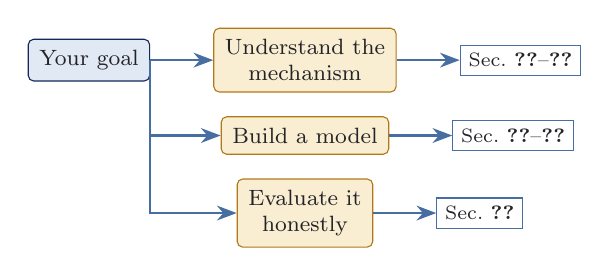
\begin{tikzpicture}[node distance=4mm]
\node[box] (goal) {Your goal};
\node[hot, right=8mm of goal] (mech) {Understand the\\mechanism};
\node[hot, below=3mm of mech] (build) {Build a model};
\node[hot, below=3mm of build] (eval) {Evaluate it\\honestly};
\node[plain, right=8mm of mech] (s34) {Sec.~\ref{sec:classical}--\ref{sec:quantum}};
\node[plain, right=8mm of build] (s5) {Sec.~\ref{sec:buildit}--\ref{sec:casestudy}};
\node[plain, right=8mm of eval] (s7) {Sec.~\ref{sec:pitfalls}};
\draw[flow] (goal.east) -- (mech.west);
\draw[flow] (goal.east) |- (build.west);
\draw[flow] (goal.east) |- (eval.west);
\draw[flow] (mech) -- (s34);
\draw[flow] (build) -- (s5);
\draw[flow] (eval) -- (s7);
\end{tikzpicture}}
\caption{Reading path. The unifying mechanism is in
Sections~\ref{sec:classical}--\ref{sec:quantum}; how to build a model in
Sections~\ref{sec:buildit}--\ref{sec:casestudy}; how to evaluate it without fooling
yourself in Section~\ref{sec:pitfalls}.}
\label{fig:reading}
\end{figure}


\section{Related Tutorials and Where This One Differs}
\label{sec:related}

Three bodies of work meet in this tutorial, and it is useful to say up front what we
borrow from each and what we add.

\textit{Graph neural networks.} Surveys of GNNs~\cite{wu2021gnnsurvey} catalog
architectures (spectral~\cite{bruna2014spectral,defferrard2016chebnet},
convolutional~\cite{kipf2017gcn}, attentional~\cite{velickovic2018gat},
message-passing~\cite{gilmer2017mpnn}, expressive~\cite{xu2019gin}, and
inductive~\cite{hamilton2017graphsage}) and their applications. A parallel line studies
the depth and range limits of these models, including over-smoothing fixes such as
deep propagation~\cite{chen2020gcnii,gasteiger2019appnp} and the over-squashing and
bottleneck phenomena that bound how far a local operator can carry
information~\cite{alon2021bottleneck,topping2022oversquashing}. We do not add to that
catalog. Instead we adopt the spectral, operator-theoretic reading of
GNNs~\cite{shuman2013gsp} and push it to its conclusion: once a layer is written as a
function of the Laplacian, the classical and quantum cases sit on the same axis.
Diffusion-based learning~\cite{gasteiger2019diffusion} is the closest classical neighbor
of our view, and dynamic-graph learning~\cite{rossi2020tgn,kazemi2020dynamicsurvey}
supplies the time-varying setting.

\textit{Quantum machine learning.} Reviews of quantum machine
learning~\cite{biamonte2017qml,dunjko2018review} and variational quantum
algorithms~\cite{cerezo2021vqa} survey models~\cite{schuld2014quest}, feature
maps~\cite{schuld2019featurespace,havlicek2019supervised}, trainability and
power~\cite{abbas2021power}, and the obstacles of the NISQ
era~\cite{preskill2018nisq,mcclean2018barren}. Quantum graph models in particular,
including quantum graph neural networks~\cite{verdon2019qgnn}, equivariant quantum graph
circuits~\cite{mernyei2022equivariant}, quantum graph
kernels~\cite{henry2021quantumkernel}, and the broad quantum-walk
literature~\cite{farhi1998quantumwalk,kempe2003qwalk,childs2003exponential,childs2004quantumwalk,childs2009universal,venegas2012quantumwalks,portugal2013book},
supply the operators we use. These works establish what is possible; they rarely
isolate, on a controlled task, what the quantum operator changes relative to a
param-matched classical one. That isolation is our contribution.

\textit{Learning for non-terrestrial networks.} The networking literature surveys
satellite systems~\cite{kodheli2021ntn}, studies low-latency routing over LEO
constellations~\cite{handley2018delay}, and provides realistic
simulators~\cite{kassing2020hypatia}. Graph and learning-based methods are by now
established for network modeling and resource
management~\cite{rusek2020routenet,shen2021gnnradio,eisen2020optimal,mao2016resource}.
We borrow the dynamic-graph setting from this line of work but deliberately keep the
task generic and the simulator minimal, so that the tutorial's conclusions are about
operators rather than about one deployment.

\textit{What is new here.} The gap these literatures leave is a single, teachable
through-line from classical message passing to quantum walks, paired with an honest
methodology for deciding whether the quantum option helps. We fill it with the
propagation-operator view (Sections~\ref{sec:classical}--\ref{sec:quantum}), a built,
runnable model (Section~\ref{sec:buildit}), a reproducible and multi-seed case study
(Section~\ref{sec:casestudy}), and a pitfall catalogue with a checklist
(Section~\ref{sec:pitfalls}). The aim is not breadth of coverage but a reader who can
both build and judge.

\section{Dynamic Wireless Topologies as Graphs}
\label{sec:background}

Fig.~\ref{fig:overview} sketches the pipeline this tutorial studies: a constellation
induces a time-varying graph, a propagation operator turns node features into a
node-level field, and the operator is the lever we vary.
\begin{figure*}[t]
\centering
\resizebox{\textwidth}{!}{%
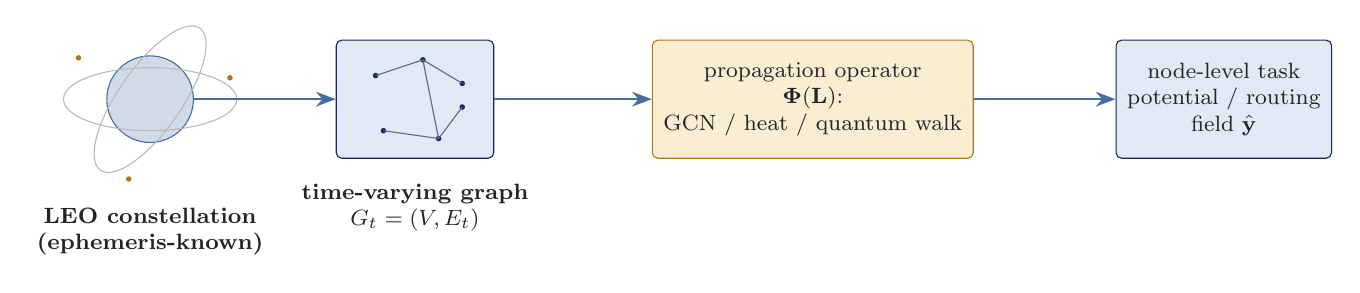
\begin{tikzpicture}[node distance=14mm]
% Stage 1: LEO constellation (Earth + satellites on two orbits)
\node[circle, draw=steel, fill=steel!25, minimum size=11mm] (earth) at (0,0) {};
\draw[gray!55] (earth.center) ellipse (11mm and 4mm);
\draw[gray!55, rotate around={55:(earth.center)}] (earth.center) ellipse (11mm and 4mm);
\foreach \a in {15,150,255}{\fill[amber!80!black] ($(earth.center)+(\a:10.5mm)$) circle (1pt);}
\node[font=\footnotesize\bfseries, text=ink, align=center, below=7mm of earth] (l1)
  {LEO constellation\\(ephemeris-known)};

% Stage 2: time-varying graph
\node[box, minimum width=20mm, minimum height=15mm, right=18mm of earth] (g) {};
\foreach \x/\y in {-5/3,1/5,6/2,-4/-4,3/-5,6/-1}{%
  \fill[navy] ($(g.center)+(\x mm,\y mm)$) circle (1pt);}
\draw[navy!70] ($(g.center)+(-5mm,3mm)$)--($(g.center)+(1mm,5mm)$)--($(g.center)+(6mm,2mm)$);
\draw[navy!70] ($(g.center)+(-4mm,-4mm)$)--($(g.center)+(3mm,-5mm)$)--($(g.center)+(6mm,-1mm)$);
\draw[navy!70] ($(g.center)+(1mm,5mm)$)--($(g.center)+(3mm,-5mm)$);
\node[font=\footnotesize\bfseries, text=ink, align=center, below=2mm of g] (l2)
  {time-varying graph\\$G_t=(V,E_t)$};

% Stage 3: operator
\node[hot, align=center, minimum width=26mm, minimum height=15mm, right=20mm of g] (op)
  {propagation operator\\$\Prop(\Lap)$:\\GCN / heat / quantum walk};

% Stage 4: task
\node[box, align=center, minimum width=22mm, minimum height=15mm, right=18mm of op] (task)
  {node-level task\\potential / routing\\field $\hat{\mathbf{y}}$};

\draw[flow] (earth.east) -- (g.west);
\draw[flow] (g.east) -- (op.west);
\draw[flow] (op.east) -- (task.west);
\end{tikzpicture}}
\caption{System overview. A LEO constellation with known future geometry induces a
time-varying graph $G_t$; a propagation operator $\Prop(\Lap)$, classical or quantum,
turns node features into a node-level field (here a potential / routing field). This
tutorial studies the choice of $\Prop$ as the lever: the operator is the only thing that
changes between classical, diffusive, and quantum, ballistic, propagation.}
\label{fig:overview}
\end{figure*}


\subsection{The time-varying graph model}
We model a network at slot $t$ as a graph $G_t=(V,E_t)$ with $|V|=N$ nodes and a
time-varying edge set $E_t$. Let $\Adj_t\in\{0,1\}^{N\times N}$ be the adjacency
matrix (or a weighted variant carrying link delay or capacity), $\Deg_t$ the diagonal
degree matrix, and
\begin{equation}
\Lap_t=\Deg_t-\Adj_t, \qquad
\Lap_t^{\mathrm{sym}}=\Id-\Deg_t^{-1/2}\Adj_t\Deg_t^{-1/2}
\end{equation}
the combinatorial and symmetric-normalized Laplacians. Each $\Lap_t$ is symmetric
positive semidefinite, with eigendecomposition $\Lap_t=\Eig_t\,\mathrm{diag}(\lambda)\,\Eig_t^{\top}$,
$\lambda_k\ge 0$. Node attributes are collected in $\mathbf{X}\in\mathbb{R}^{N\times d}$.
Table~\ref{tab:notation} summarizes the notation used throughout.

A defining feature of LEO and other non-terrestrial
networks~\cite{kodheli2021ntn,handley2018delay} is that the future
topology is \emph{known}: orbits are deterministic over the analysis horizon, so
$\Adj_{t+1},\Adj_{t+2},\dots$ can be computed in advance from ephemeris. This is
unusual among dynamic graphs and is worth keeping in mind, although the case study
in this tutorial uses only a single snapshot per sample to keep the exposition focused
on the operator question.

\subsection{Learning tasks on $G_t$}
Many network-management problems become node-level or edge-level learning tasks once
the topology is a graph:
\begin{itemize}
\item \emph{Potential and reachability fields}: predict, for every node, a scalar
that encodes distance or reachability to a target. This underlies routing and
forwarding and is the task we use in the case study.
\item \emph{Traffic and congestion}: predict link load or a congestion price for
resource-aware forwarding.
\item \emph{Anomaly and security}: classify nodes or subgraphs as anomalous under
shifting topology.
\end{itemize}
What these share is a need to move information across the graph. How far and how fast
that information should move is exactly the property that distinguishes propagation
operators, which is why the choice of operator, not the choice of task, is the right
lever to study first.

\subsection{What makes these graphs hard}
Three features set dynamic wireless graphs apart from the static citation and molecule
graphs on which GNNs are usually taught. First, \emph{churn}: edges appear and disappear
between slots as satellites cross polar regions or seams, so an operator that overfits a
single topology generalizes poorly. Second, \emph{large diameter}: a constellation graph
is locally grid-like and globally sparse, so geodesics are long and a fixed-hop operator
is starved of range exactly where it is needed. Third, \emph{scale with structure}:
realistic shells have thousands of nodes but a regular plane-and-seam structure, which
both stresses computation and offers regularity an inductive operator can exploit. The
node-potential task we study isolates the second feature, range, because it is the one
the propagation operator most directly controls; the others motivate the roadmap in
Section~\ref{sec:roadmap}.

\begin{table}[t]
\centering
\caption{Notation used throughout the tutorial.}
\label{tab:notation}
\renewcommand{\arraystretch}{1.15}
\begin{tabular}{@{}ll@{}}
\toprule
Symbol & Meaning \\
\midrule
$G_t=(V,E_t)$ & graph at slot $t$, $N=|V|$ nodes \\
$\Adj_t,\Deg_t,\Lap_t$ & adjacency, degree, Laplacian \\
$\Eig,\lambda_k$ & Laplacian eigenvectors and eigenvalues \\
$\mathbf{X},\Feat^{(\ell)}$ & input features, layer-$\ell$ embeddings \\
$\Prop(\Lap)$ & propagation operator (the unifying object) \\
$t_\ell$ & learnable propagation time at layer $\ell$ \\
$\Wt^{(\ell)}$ & learnable layer weights \\
$\mathrm{ecc}(v),\,\mathrm{diam}(G)$ & eccentricity of $v$, graph diameter \\
\bottomrule
\end{tabular}
\end{table}

\section{A Survey of Graph Learning for Wireless Networks, by Operator}
\label{sec:survey}

Having fixed the propagation-operator view, we use it to organize the landscape.
Fig.~\ref{fig:taxonomy} is the map: every method we discuss is a choice of operator
$\Prop(\Lap)$, optionally wrapped to handle a time-varying graph. This section surveys
the four branches and their use in wireless and non-terrestrial networks; the depth on
each is intentionally uneven, favoring the operators we later build and test.

\begin{figure*}[t]
\centering
\resizebox{\textwidth}{!}{%
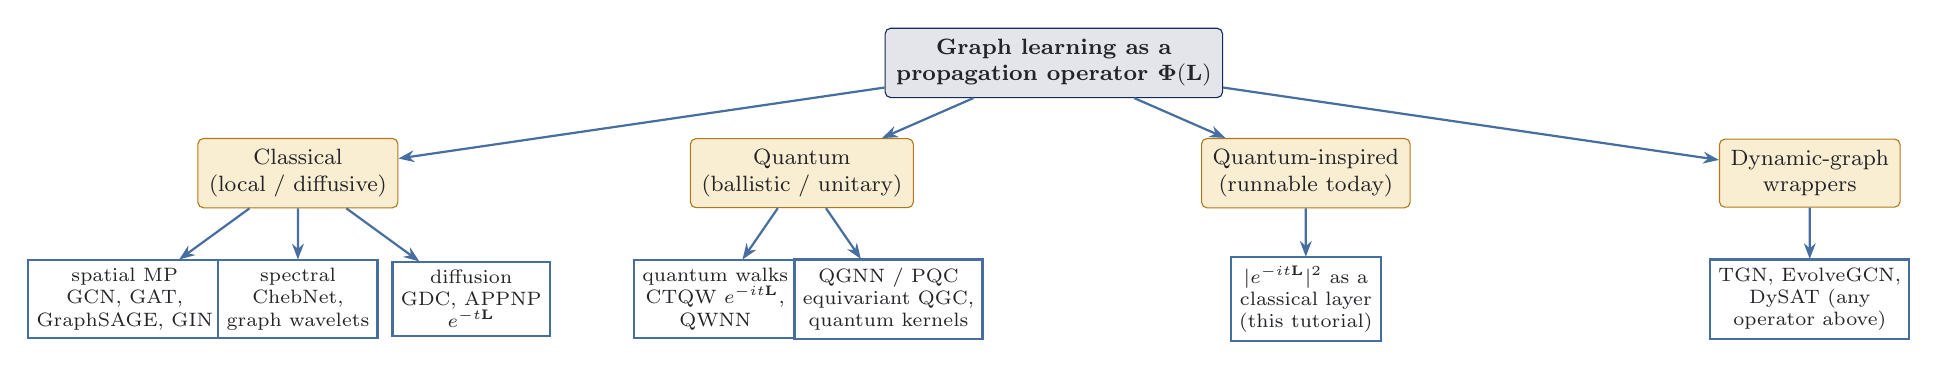
\begin{tikzpicture}[
  every node/.style={font=\footnotesize},
  root/.style={box, fill=navy!12, draw=navy, font=\footnotesize\bfseries},
  fam/.style={hot, align=center},
  leaf/.style={plain, align=center, font=\scriptsize},
  edge from parent/.style={draw=steel, thick, -{Stealth[length=2mm]}},
  level 1/.style={sibling distance=64mm, level distance=14mm},
  level 2/.style={sibling distance=22mm, level distance=16mm},
]
\node[root] {Graph learning as a\\propagation operator $\Prop(\Lap)$}
  child {node[fam] {Classical\\(local / diffusive)}
    child {node[leaf] {spatial MP\\GCN, GAT,\\GraphSAGE, GIN}}
    child {node[leaf] {spectral\\ChebNet,\\graph wavelets}}
    child {node[leaf] {diffusion\\GDC, APPNP\\$e^{-t\Lap}$}}
  }
  child {node[fam] {Quantum\\(ballistic / unitary)}
    child {node[leaf] {quantum walks\\CTQW $e^{-it\Lap}$,\\QWNN}}
    child {node[leaf] {QGNN / PQC\\equivariant QGC,\\quantum kernels}}
  }
  child {node[fam] {Quantum-inspired\\(runnable today)}
    child {node[leaf] {$|e^{-it\Lap}|^2$ as a\\classical layer\\(this tutorial)}}
  }
  child {node[fam] {Dynamic-graph\\wrappers}
    child {node[leaf] {TGN, EvolveGCN,\\DySAT (any\\operator above)}}
  };
\end{tikzpicture}}
\caption{A taxonomy of graph learning organized by the propagation operator
$\Prop(\Lap)$. Classical operators are local (spatial message passing) or diffusive
(spectral / heat); quantum operators are unitary and ballistic (continuous-time quantum
walks, parameterized quantum graph circuits); the quantum-inspired branch runs the
quantum-walk kernel on classical hardware; dynamic-graph wrappers compose with any
operator to handle a time-varying topology. This tutorial threads the classical,
quantum, and quantum-inspired branches onto one axis.}
\label{fig:taxonomy}
\end{figure*}


\subsection{Classical operators}
The spatial branch of message passing, GCN~\cite{kipf2017gcn},
GraphSAGE~\cite{hamilton2017graphsage}, GAT~\cite{velickovic2018gat},
GIN~\cite{xu2019gin}, and the general message-passing framework~\cite{gilmer2017mpnn},
shares a $K$-hop horizon and is surveyed comprehensively
elsewhere~\cite{wu2021gnnsurvey,zhou2020gnnreview,bronstein2017geometric}. The spectral
branch, rooted in graph signal processing~\cite{shuman2013gsp,ortega2018gsp} and spectral
graph theory~\cite{chung1997spectral}, expresses a layer as a function of $\Lap$:
ChebNet~\cite{defferrard2016chebnet} and graph wavelets~\cite{hammond2011wavelets} are
polynomials of the spectrum, while the diffusion branch
(GDC~\cite{gasteiger2019diffusion}, APPNP~\cite{gasteiger2019appnp},
GCNII~\cite{chen2020gcnii}) uses the heat kernel $e^{-t\Lap}$ or its rational cousins to
propagate globally. The recurring failure mode of the local branch, the inability to
carry information past the depth horizon, is studied as over-smoothing~\cite{li2018deeper}
and over-squashing~\cite{alon2021bottleneck,topping2022oversquashing}; it is exactly the
deficiency our case study exposes.

\subsection{Quantum and quantum-inspired operators}
The quantum branch replaces dissipative diffusion by unitary evolution. Continuous-time
quantum walks~\cite{farhi1998quantumwalk,childs2004quantumwalk}, reviewed
in~\cite{kempe2003qwalk,venegas2012quantumwalks,portugal2013book}, underlie quantum
speedups~\cite{childs2003exponential} and are computationally
universal~\cite{childs2009universal}; their learning incarnation is the quantum-walk
neural network~\cite{dernbach2019qwnn}. The parameterized-circuit branch encodes graph
features into qubits and learns with variational
circuits~\cite{mitarai2018qcl,farhi2018classification,cerezo2021vqa}: quantum graph
neural networks~\cite{verdon2019qgnn}, equivariant quantum graph
circuits~\cite{mernyei2022equivariant}, and quantum graph kernels~\cite{henry2021quantumkernel}.
Their appeal is the exponential-dimensional feature
map~\cite{schuld2019featurespace,havlicek2019supervised,schuld2018book} and, in some
settings, provable data or speed advantages~\cite{huang2021power,liu2021rigorous};
their obstacles are NISQ noise~\cite{preskill2018nisq}, barren
plateaus~\cite{mcclean2018barren}, and limited qubits, surveyed
in~\cite{biamonte2017qml,dunjko2018review}. The quantum-inspired branch sidesteps the
hardware by running the quantum-walk kernel $|e^{-it\Lap}|^2$ as a classical layer; it is
the operator we build and evaluate, and Table~\ref{tab:opfamilies} places it against the
others.

\subsection{Handling the time-varying topology}
Any operator above can be wrapped to track a changing graph. Dynamic-graph
methods~\cite{kazemi2020dynamicsurvey} such as TGN~\cite{rossi2020tgn},
EvolveGCN~\cite{pareja2020evolvegcn}, and DySAT~\cite{sankar2020dysat} learn over a
sequence of snapshots; for LEO networks the future graph is moreover known from
ephemeris, a structure most of these methods do not exploit and that we flag as an
opportunity in Section~\ref{sec:roadmap}.

\begin{table}[t]
\centering
\caption{Operator families on the propagation axis. $N$ nodes, $|E|$ edges,
$K$ layers/hops, $d$ feature width.}
\label{tab:opfamilies}
\renewcommand{\arraystretch}{1.25}
\footnotesize
\begin{tabular}{@{}p{0.20\columnwidth}p{0.20\columnwidth}p{0.16\columnwidth}p{0.18\columnwidth}@{}}
\toprule
Family & Operator $\Prop$ & Reach / spread & Cost (layer) \\
\midrule
Spatial MP & $\hat{\Adj}$ (1-hop) & local, $K$ hops & $O(|E|d)$ \\
Diffusion & $e^{-t\Lap}$ & global, $\sim\!\sqrt{t}$ & $O(N^3)$ eig$^\dagger$ \\
Quantum walk & $e^{-it\Lap}$ (unitary) & global, $\sim\! t$ & $O(N^3)$ eig$^\dagger$ \\
Quantum-inspired & $|e^{-it\Lap}|^2$ & global, $\sim\! t$ & $O(N^3)$ eig$^\dagger$ \\
True QGNN/PQC & PQC on qubits & Hilbert-space & NISQ-limited \\
\bottomrule
\end{tabular}
\\[2pt]
{\footnotesize $^\dagger$ amortized over layers; reducible to $O(|E|)$ per
matrix-vector product with Chebyshev/Krylov approximation (Section~\ref{sec:roadmap}).}
\end{table}

\subsection{Graph and quantum learning in wireless and non-terrestrial networks}
On the application side, graph learning is now established for communication
networks~\cite{suarezvarela2023gnn,jiang2022graph}; we group the uses by the task they
place on the graph.

\emph{Routing and traffic engineering.} The earliest and most direct use treats the
network as a graph and learns to predict path-level quantities. RouteNet models per-path
delay, jitter, and loss and uses the learned model to optimize
routing~\cite{rusek2020routenet}; the appeal is that a graph model generalizes across
topologies a per-topology optimizer cannot reuse. This is the regime where the local
versus global operator distinction of this tutorial bites hardest, because routing
potentials are long-range fields on a large-diameter graph.

\emph{Resource management and physical layer.} A second line learns resource-allocation
and power-control policies as functions on the interference or connectivity graph, where
permutation-equivariant graph operators give scalability and transferability that dense
networks lack~\cite{shen2021gnnradio,eisen2020optimal}, frequently combined with
reinforcement learning for sequential control~\cite{mao2016resource}. Here the graph is
often denser and lower-diameter, so a local operator can suffice, a useful contrast to
the routing regime that the operator view makes explicit.

\emph{Non-terrestrial and satellite networks.} LEO
mega-constellations~\cite{delportillo2019technical} are the setting of our case study:
they pose low-latency routing over a fast-moving but ephemeris-predictable
topology~\cite{handley2018delay}, with packet-level simulators available for honest
evaluation~\cite{kassing2020hypatia}. Because the constellation is physically distributed
and bandwidth to the ground is scarce, learning is increasingly pushed on board and
across satellites through federated schemes~\cite{razmi2022board,matthiesen2024federated},
which raises the decentralization question we return to in Section~\ref{sec:roadmap}.

\emph{Quantum methods for networking.} Quantum techniques enter this space along two
routes: quantum search and optimization for discrete network functions such as
virtualization and routing~\cite{botsinis2019quantum}, and the longer-term
quantum-internet vision in which entanglement distribution is itself a network
service~\cite{wehner2018quantum}. Graph-structured quantum learning, the subject of this
tutorial, sits between them: a learned propagation operator rather than a fixed search
subroutine.

Table~\ref{tab:qgraphworks} summarizes representative quantum graph-learning works by how
they encode the graph and what they target. The gap this tutorial fills is the
controlled, honest comparison of these operators on a single dynamic-wireless task, which
the application literature above rarely isolates.

\begin{table}[t]
\centering
\caption{Representative quantum / quantum-inspired graph-learning works by encoding and
target. Sim = classical simulation; HW = quantum hardware.}
\label{tab:qgraphworks}
\renewcommand{\arraystretch}{1.25}
\footnotesize
\begin{tabular}{@{}p{0.27\columnwidth}p{0.30\columnwidth}p{0.18\columnwidth}@{}}
\toprule
Work & Mechanism / encoding & Realization \\
\midrule
CTQW~\cite{childs2004quantumwalk} & unitary $e^{-it\Lap}$, search & theory \\
QWNN~\cite{dernbach2019qwnn} & learned-coin quantum walk & Sim \\
QGNN~\cite{verdon2019qgnn} & Hamiltonian-based PQC & Sim \\
EQGC~\cite{mernyei2022equivariant} & equivariant graph circuit & Sim \\
Quantum kernel~\cite{henry2021quantumkernel} & evolution kernel, qubit array & Sim/HW \\
This tutorial & $|e^{-it\Lap}|^2$ classical layer & Sim (CPU) \\
\bottomrule
\end{tabular}
\end{table}

\section{Classical Graph Neural Networks as Propagation}
\label{sec:classical}

\subsection{Message passing is local propagation}
A graph convolutional network (GCN) layer~\cite{kipf2017gcn,defferrard2016chebnet}
updates node embeddings by averaging over neighbors and applying a learned linear map
and nonlinearity,
\begin{equation}
\Feat^{(\ell+1)}=\sigma\!\big(\hat{\Adj}\,\Feat^{(\ell)}\Wt^{(\ell)}\big),\qquad
\hat{\Adj}=\tilde{\Deg}^{-1/2}\tilde{\Adj}\,\tilde{\Deg}^{-1/2},
\end{equation}
where $\tilde{\Adj}=\Adj+\Id$ adds self-loops and $\tilde{\Deg}$ is its degree matrix.
The operator $\hat{\Adj}$ is a degree-one polynomial in the adjacency, so one layer
mixes one hop and $K$ stacked layers mix exactly $K$ hops. This locality is the key
structural fact about GCNs: a $K$-layer GCN simply cannot move information farther
than $K$ hops, regardless of width.

\subsection{The continuous view: diffusion}
Stacking many small averaging steps approaches a continuous diffusion. The heat
equation on a graph, $\dot{\mathbf{x}}=-\Lap\mathbf{x}$, has the closed-form solution
\begin{equation}
\mathbf{x}(t)=e^{-t\Lap}\,\mathbf{x}(0),\qquad
e^{-t\Lap}=\Eig\,\mathrm{diag}\!\big(e^{-t\lambda_k}\big)\,\Eig^{\top}.
\label{eq:heat}
\end{equation}
Because $\Lap\mathbf{1}=\mathbf{0}$, the kernel $e^{-t\Lap}$ is row-stochastic and
nonnegative: it is a genuine probability kernel that smooths a signal across the
whole graph, with a single scalar $t$ controlling how far. A diffusion-based GNN
layer~\cite{gasteiger2019diffusion} replaces $\hat{\Adj}$ by $e^{-t\Lap}$ and, unlike a
fixed $K$-hop GCN, can reach any node at the cost of a learnable time $t$. Other local
message-passing schemes~\cite{hamilton2017graphsage,velickovic2018gat} share the same
$K$-hop horizon.

\subsection{Why range matters}
The defining property of diffusion is \emph{how fast it spreads}. For an impulse
released at a node, the spatial second moment of the heat kernel grows linearly in
time,
\begin{equation}
\Var\big[e^{-t\Lap}\big]\;\sim\;t .
\label{eq:diffusive}
\end{equation}
This linear, diffusive spreading is the classical baseline against which we will
contrast the quantum walk. It already tells us what to expect from the case study:
on tasks that require long-range information, a global diffusion operator should beat
a local $K$-hop GCN, simply because it can reach the far nodes at all. The interesting
question is what, if anything, a quantum operator adds beyond reaching them.

\paragraph*{Worked example} Take a path of $N=81$ nodes and release an impulse at the
center. The heat kernel $e^{-t\Lap}$ gives a Gaussian-like profile whose spatial
variance is exactly $2t$: at $t=1$ the variance is $2$, at $t=4$ it is $8$, and at
$t=8$ it is $16$ (the steel curve in Fig.~\ref{fig:expA}). The mass reaches farther as
$t$ grows, but only as $\sqrt{t}$ in distance. A $K$-layer GCN, by contrast, places
exactly zero mass beyond hop $K$ no matter how it is trained; on this path a $3$-layer
GCN can never see node $40$ from the center. This is the concrete sense in which range,
not capacity, is the limiting resource for local operators.

\section{Quantum and Quantum-Inspired Graph Models}
\label{sec:quantum}

\subsection{Continuous-time quantum walks}
The continuous-time quantum walk
(CTQW)~\cite{childs2004quantumwalk,venegas2012quantumwalks} is the quantum analogue of
graph diffusion. Replacing the real, dissipative dynamics of the heat equation by the
complex, unitary Schr\"odinger dynamics gives
\begin{equation}
\begin{aligned}
i\,\dot{\boldsymbol{\psi}}=\Lap\boldsymbol{\psi}
\;\;\Longrightarrow\;\;
\boldsymbol{\psi}(t)&=e^{-it\Lap}\boldsymbol{\psi}(0),\\[2pt]
e^{-it\Lap}&=\Eig\,\mathrm{diag}\!\big(e^{-it\lambda_k}\big)\,\Eig^{*}.
\end{aligned}
\label{eq:qwalk}
\end{equation}
The operator $e^{-it\Lap}$ is \emph{unitary} rather than stochastic, so it preserves
the norm of the state and produces interference between paths.

\textit{Interference, intuitively.} In classical diffusion, the contributions of two
walks that reach the same node always add as nonnegative probabilities, so spreading is
a smooth averaging that loses height as it widens. In a quantum walk the contributions
are complex amplitudes that carry a phase, so two walks reaching the same node can add
constructively or cancel. Constructive interference along the graph's geodesics is what
lets probability mass race outward in a coherent front rather than diffuse, and
destructive interference is what produces the oscillatory tails visible in
Fig.~\ref{fig:operators}. The price of this coherence is fragility: any decoherence,
whether physical device noise or, in the classical surrogate, an averaging that washes
out phase, collapses the quantum walk back toward diffusion. This is the same fragility
we see empirically as higher seed-to-seed variance in Section~\ref{sec:casestudy}.

The physically meaningful quantity is the transition probability,
\begin{equation}
\Prop_{\mathrm{qw}}(t)_{ij}=\big|[e^{-it\Lap}]_{ij}\big|^2 ,
\label{eq:qwprob}
\end{equation}
which is again real and row-stochastic, so it plugs into the same layer template as
the heat kernel and stays param-matched with it.

\subsection{The one difference that matters: ballistic spreading}
Interference changes the spreading law. Whereas the heat kernel spreads diffusively,
\eqref{eq:diffusive}, the quantum walk spreads \emph{ballistically}:
\begin{equation}
\Var\big[\,|e^{-it\Lap}|^2\big]\;\sim\;t^2 .
\label{eq:ballistic}
\end{equation}
The probability mass reaches distant nodes quadratically faster in propagation time.

\paragraph*{Worked example, continued} On the same $81$-node path and impulse, the
quantum-walk probability $|e^{-it\Lap}|^2$ has variance exactly $2t^2$: at $t=1$ it is
$2$ (the same as heat), at $t=4$ it is $32$ (four times heat), and at $t=8$ it is $128$
(eight times heat). The two operators agree at $t=1$ and then separate, the quantum
walk pulling ahead as $t^2$ versus $t$ (Fig.~\ref{fig:expA}). The distance frontier
advances linearly in $t$ for the walk but only as $\sqrt{t}$ for diffusion. This is the
entire mechanistic claim, and it is exact, not statistical; the open question is whether
it survives into an end-task gain once weights and a readout are trained on top.

Fig.~\ref{fig:operators} summarizes the whole framework: one Laplacian, three
operators, two spreading laws. This is the single, measurable sense in which the
quantum walk differs from classical diffusion, and Section~\ref{sec:casestudy}
verifies \eqref{eq:diffusive} and \eqref{eq:ballistic} directly.

\begin{figure*}[t]
\centering
\resizebox{\textwidth}{!}{%
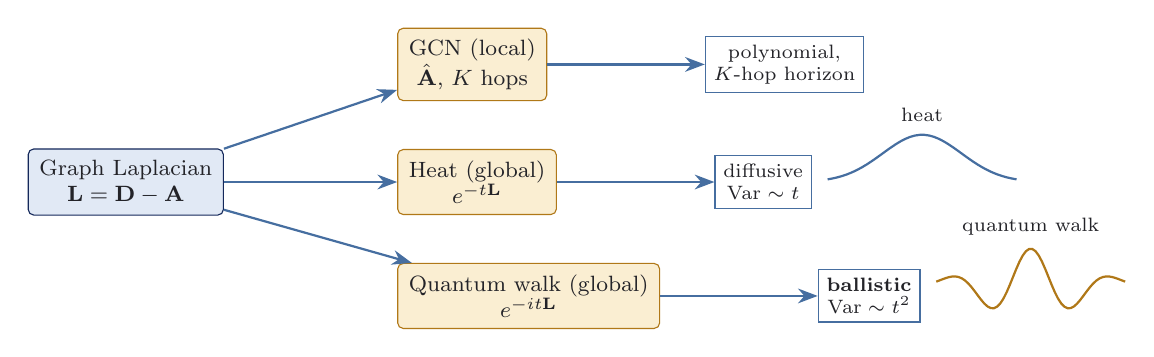
\begin{tikzpicture}[node distance=6mm]
% center: the Laplacian
\node[box, minimum width=22mm] (lap) {Graph Laplacian\\$\Lap=\Deg-\Adj$};

% three operators
\node[hot, above right=6mm and 22mm of lap] (gcn) {GCN (local)\\$\hat{\Adj}$, $K$ hops};
\node[hot, right=22mm of lap] (heat) {Heat (global)\\$e^{-t\Lap}$};
\node[hot, below right=6mm and 22mm of lap] (qw) {Quantum walk (global)\\$e^{-it\Lap}$};

\draw[flow] (lap) -- (gcn);
\draw[flow] (lap) -- (heat);
\draw[flow] (lap) -- (qw);

% spreading law annotations
\node[plain, right=20mm of gcn] (gcns) {polynomial,\\$K$-hop horizon};
\node[plain, right=20mm of heat] (heats) {diffusive\\$\Var\sim t$};
\node[plain, right=20mm of qw] (qws) {\textbf{ballistic}\\$\Var\sim t^2$};

\draw[flow] (gcn) -- (gcns);
\draw[flow] (heat) -- (heats);
\draw[flow] (qw) -- (qws);

% mini spreading sketches
\begin{scope}[shift={($(heats.east)+(14mm,0)$)}]
  \draw[steel, thick] plot[domain=-1.2:1.2, samples=40]
       (\x, {0.6*exp(-2*\x*\x)});
  \node[font=\scriptsize, text=ink, above] at (0,0.65) {heat};
\end{scope}
\begin{scope}[shift={($(qws.east)+(14mm,0)$)}]
  \draw[amber!80!black, thick] plot[domain=-1.2:1.2, samples=60]
       (\x, {0.45*(cos(deg(6*\x))*exp(-1.5*\x*\x))+0.15});
  \node[font=\scriptsize, text=ink, above] at (0,0.65) {quantum walk};
\end{scope}
\end{tikzpicture}}
\caption{The unifying view. One Laplacian, three propagation operators, two spreading
laws. The only fundamental difference between classical diffusion and the quantum walk
is diffusive ($\Var\sim t$) versus ballistic ($\Var\sim t^2$) spreading; everything
else in the network is shared, which makes the operators param-matched.}
\label{fig:operators}
\end{figure*}


\subsection{From walks to quantum graph neural networks}
A full quantum graph neural network (QGNN) goes further than a walk. Node features
are encoded into qubits, graph-structured entangling layers (a parameterized quantum
circuit, PQC) play the role of message passing, and measurements form the readout. Four
designs map out the space. \emph{Hamiltonian QGNNs}~\cite{verdon2019qgnn} build the layer
from $e^{-iH_G t}$ for a graph Hamiltonian $H_G$ with trainable couplings, the closest
relative of the quantum walk and the most direct realization of the operator view.
\emph{Quantum-walk neural networks}~\cite{dernbach2019qwnn} make the walk's coin
operator feature-dependent and learnable, so the propagation itself adapts to the data.
\emph{Equivariant quantum graph circuits}~\cite{mernyei2022equivariant} enforce
permutation equivariance in the circuit, the quantum analogue of the symmetry that makes
classical GNNs generalize across node orderings. \emph{Quantum graph
kernels}~\cite{henry2021quantumkernel} skip end-to-end learning and instead use a quantum
evolution to define a similarity between graphs that a classical model then consumes,
which is attractive because it sidesteps barren plateaus. The promise across all four is
twofold: ballistic propagation as above, and an exponentially large Hilbert-space feature
map~\cite{schuld2019featurespace,havlicek2019supervised} that a classical model cannot
represent compactly.
The cost is equally real, and we return to it in Section~\ref{sec:roadmap}: present
quantum hardware is noisy, qubit-limited, and prone to barren plateaus that flatten
the trainable landscape.

\subsection{Encodings and expressivity (a primer)}
A QGNN needs the graph and its features inside a quantum state, and the encoding choice
drives both expressivity and trainability. Three families recur. \emph{Basis encoding}
writes a length-$N$ signal into $\lceil\log_2 N\rceil$ qubits, the convention our
noise study uses, so a walk on $N$ nodes costs only logarithmically many qubits but needs
a unitary that realizes $e^{-it\Lap}$. \emph{Angle encoding} maps each feature to a
rotation angle, one qubit per feature, and is the workhorse of variational quantum
circuits~\cite{mitarai2018qcl,farhi2018classification}. \emph{Amplitude encoding} packs a
normalized feature vector into the amplitudes of a state, exponentially compact but
expensive to prepare. Table~\ref{tab:encodings} contrasts the three.

\begin{table}[t]
\centering
\caption{Quantum feature encodings for a length-$N$ signal.}
\label{tab:encodings}
\renewcommand{\arraystretch}{1.25}
\footnotesize
\begin{tabular}{@{}p{0.20\columnwidth}p{0.16\columnwidth}p{0.18\columnwidth}p{0.20\columnwidth}@{}}
\toprule
Encoding & Qubits & Prep cost & Typical use \\
\midrule
Basis & $\lceil\log_2 N\rceil$ & low (a basis state) & walks, search (our Exp~D) \\
Angle & $O(N)$ & low (one rotation each) & variational circuits \\
Amplitude & $\lceil\log_2 N\rceil$ & high (state prep) & compact feature maps \\
\bottomrule
\end{tabular}
\end{table} The promise of these encodings is a feature map into a Hilbert
space whose dimension grows exponentially with the qubit
count~\cite{schuld2019featurespace,havlicek2019supervised,schuld2018book}, where a linear
decision boundary can separate data that is hard to separate classically, and in
restricted settings this yields provable data or sample
advantages~\cite{huang2021power,liu2021rigorous,abbas2021power}. The catch is that the
same expressivity makes the training landscape flat: random deep circuits exhibit barren
plateaus where gradients vanish exponentially in the number of
qubits~\cite{mcclean2018barren}, so expressivity and trainability trade off. For a
practitioner the takeaway is that a quantum graph model is not automatically better; its
advantage, if any, depends on a careful encoding and a problem whose structure the
encoding actually exploits, which is precisely what a controlled, honest evaluation is
meant to detect.

\subsection{Quantum-inspired: the runnable middle ground}
Between a classical GCN and a fault-tolerant QGNN sits the option we recommend for
near-term practice. The quantum-walk kernel \eqref{eq:qwprob} is just a matrix
function of the Laplacian; it can be computed on a classical processor with one
eigendecomposition and used as a propagation layer. This \emph{quantum-inspired}
GNN keeps the ballistic spreading mechanism while remaining trainable and
reproducible today. It is the operator we build in the next section and evaluate in
the case study. Whether its ballistic mechanism translates into an end-task advantage
is precisely the empirical question we refuse to answer by assertion.

\section{Build It: A Quantum-Inspired GNN Layer}
\label{sec:buildit}

We now assemble a concrete, param-matched model. The design principle is that all
three operators share architecture and differ \emph{only} in $\Prop$, so any
performance gap is attributable to the operator and not to capacity.

\subsection{The shared layer}
Given layer embeddings $\Feat^{(\ell)}$, every model computes
\begin{equation}
\Feat^{(\ell+1)}=\sigma\!\big(\Prop^{(\ell)}\,\Feat^{(\ell)}\,\Wt^{(\ell)}+\mathbf{b}^{(\ell)}\big),
\end{equation}
and differs only in the operator:
\begin{align}
\text{GCN:}&\quad \Prop^{(\ell)}=\hat{\Adj}\ \text{(fixed)},\\
\text{Heat:}&\quad \Prop^{(\ell)}=\Eig\,\mathrm{diag}(e^{-t_\ell\lambda})\,\Eig^{\top},\\
\text{QI:}&\quad \Prop^{(\ell)}=\big|\Eig\,\mathrm{diag}(e^{-it_\ell\lambda})\,\Eig^{*}\big|^2 .
\end{align}
The heat and quantum-inspired (QI) operators add one learnable scalar $t_\ell$ per
layer, which is negligible against the weight matrices, so the three models have
essentially identical parameter counts. Because $\Prop$ is built from the eigenvalues
$\lambda$ with differentiable functions, $t_\ell$ trains by ordinary backpropagation;
a single eigendecomposition of $\Lap$ per graph is reused across layers and operators.

\subsection{Algorithm}
Algorithm~\ref{alg:qignn} gives the QI-GNN forward pass; the heat and GCN variants
are the same template with their operator substituted. Fig.~\ref{fig:qignn} shows the
data flow.

\begin{algorithm}[t]
\caption{QI-GNN forward pass (one graph)}
\label{alg:qignn}
\begin{algorithmic}[1]
\REQUIRE features $\mathbf{X}$; eigenpairs $(\lambda,\Eig)$ of $\Lap$;
parameters $\{t_\ell,\Wt^{(\ell)},\mathbf{b}^{(\ell)}\}_{\ell=0}^{K-1}$
\STATE $\Feat\leftarrow\mathbf{X}$
\FOR{$\ell=0$ to $K-1$}
  \STATE $\Prop\leftarrow\big|\Eig\,\mathrm{diag}(e^{-i\,t_\ell\lambda})\,\Eig^{*}\big|^2$
         \hfill\COMMENT{quantum-walk probability kernel}
  \STATE $\Feat\leftarrow\sigma\big(\Prop\,\Feat\,\Wt^{(\ell)}+\mathbf{b}^{(\ell)}\big)$
\ENDFOR
\RETURN $\mathrm{readout}(\Feat)$
\end{algorithmic}
\end{algorithm}

\begin{figure}[t]
\centering
\resizebox{\columnwidth}{!}{%
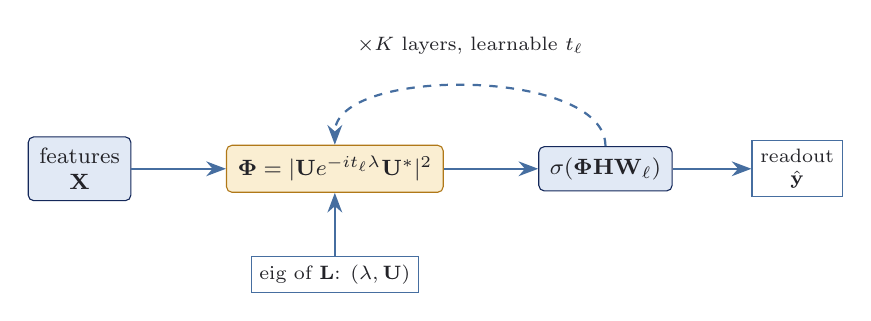
\begin{tikzpicture}[node distance=5mm]
% main horizontal data flow (clean line, no box in the way)
\node[box] (x) {features\\$\mathbf{X}$};
\node[hot, right=12mm of x] (prop) {$\Prop=|\Eig e^{-it_\ell\lambda}\Eig^{*}|^2$};
\node[box, right=12mm of prop] (mix) {$\sigma(\Prop\Feat\Wt_\ell)$};
\node[plain, right=10mm of mix] (out) {readout\\$\hat{\mathbf{y}}$};
% eigendecomposition feeds the operator from below
\node[plain, below=8mm of prop] (eig) {eig of $\Lap$: $(\lambda,\Eig)$};

\draw[flow] (x) -- (prop);
\draw[flow] (eig) -- (prop);
\draw[flow] (prop) -- (mix);
\draw[flow] (mix) -- (out);
% recurrence over K layers: arc well above the boxes, label above the arc
\draw[flow, dashed] (mix.north) .. controls +(0,10mm) and +(0,10mm) .. (prop.north);
\node[font=\scriptsize, text=ink, above=1pt]
  at ($(prop.north)!0.5!(mix.north) + (0,10mm)$)
  {$\times K$ layers, learnable $t_\ell$};
\end{tikzpicture}}
\caption{QI-GNN data flow (Algorithm~\ref{alg:qignn}). The quantum-walk kernel is
built once from the Laplacian spectrum (fed in from below) and reused across $K$ layers;
the heat and GCN variants substitute their operator into the same template, keeping the
models param-matched.}
\label{fig:qignn}
\end{figure}


\subsection{Design variants}
The quantum-walk family has design knobs worth knowing, which we probe empirically in
Section~\ref{sec:casestudy}: the walk can run on the adjacency $e^{-it\Adj}$ or the
normalized Laplacian $e^{-it\Lap^{\mathrm{sym}}}$ instead of $\Lap$, and a layer can
concatenate several learnable times $\{t_{\ell,m}\}$ for a multi-time readout. These
are alternatives a practitioner would naturally try when seeking an advantage, so we
test them rather than assume one of them is best.

\subsection{A worked micro-example}
To make the operator concrete, take the $3$-node path $1\!-\!2\!-\!3$ with combinatorial
Laplacian
\begin{equation}
\Lap=\begin{pmatrix} 1 & -1 & 0\\ -1 & 2 & -1\\ 0 & -1 & 1\end{pmatrix},
\quad \text{eigenvalues } \lambda\in\{0,1,3\}.
\end{equation}
Seeding the centre node and propagating for a small time $t$, the heat kernel keeps the
mass concentrated near the centre and merely leaks symmetrically outward, whereas the
quantum-walk probability $|e^{-it\Lap}|^2$ develops oscillatory amplitude that, as $t$
grows, pushes weight onto the two endpoints faster than diffusion would. On this tiny
graph the difference is modest, but it is the same mechanism that, scaled to a constellation
of large diameter, separates a global operator from a local one and produces the far-node
behavior measured in Section~\ref{sec:casestudy}. In code, the entire layer is the three
lines of Algorithm~\ref{alg:qignn}: form the eigenpairs once, build $\Prop$ from a
learnable $t_\ell$, and apply $\sigma(\Prop\Feat\Wt_\ell)$.

\subsection{Cost}
The three operators differ in cost as well as physics. The GCN operator $\hat{\Adj}$ is
sparse, so a layer costs $O(|E_t|\,d)$ for $d$-dimensional features. The heat and
quantum-walk kernels are dense $N\times N$ matrices built from one symmetric
eigendecomposition per graph, an $O(N^3)$ step that dominates at our scale but is shared
across layers and across all spectral operators, so it is amortized. For the hundreds of
nodes in the case study this is a fraction of a second on a CPU. It does not scale to
thousands of satellites, which is why Section~\ref{sec:roadmap} turns to
Krylov-subspace and Chebyshev approximations that compute the action $e^{-it\Lap}\Feat$
without ever forming the full kernel or its spectrum. The practical takeaway is that the
quantum-inspired operator carries no training-time penalty relative to classical
diffusion: they share the same bottleneck.

\subsection{A practical recipe}
To apply this framework to a new dynamic-wireless task, the following recipe captures the
whole workflow. (1) \emph{Build the graph}: define $G_t$ from the network state, the
adjacency by physical or logical links, and choose features that the operator can
propagate (for a potential field, a one-hot source plus a normalized degree suffices).
(2) \emph{Pick the operator by range}: if the task is short-range, start with a $K$-layer
GCN; if it is long-range on a large-diameter graph, use a global operator and treat the
classical heat kernel as the default. (3) \emph{Add the quantum-inspired option as an
ablation}, not as the hero: include $|e^{-it\Lap}|^2$ and, if you pursue it, sweep its
base matrix (adjacency, Laplacian, normalized Laplacian) as in Exp~B2. (4) \emph{Keep it
param-matched}: vary only the operator, holding depth, width, and weight shapes fixed.
(5) \emph{Evaluate honestly}: multiple seeds with mean and standard deviation, a
scale-free metric (AURC), honest denominators, and a verdict that treats any within-noise
ranking as a tie. (6) \emph{Scale with care}: replace the $O(N^3)$ eigendecomposition by a
Chebyshev or Krylov approximation of $e^{-it\Lap}\Feat$ before going to thousands of
nodes. The case study in Section~\ref{sec:casestudy} is a worked instance of exactly this
recipe.

\section{A Reproducible LEO Case Study}
\label{sec:casestudy}

The case study comprises five experiments, summarized in Table~\ref{tab:expsummary};
each isolates one question, from the bare mechanism to scale and hardware noise, and each
is reproducible from seeded runs in the companion code.

\begin{table}[t]
\centering
\caption{The five case-study experiments and what each isolates.}
\label{tab:expsummary}
\renewcommand{\arraystretch}{1.25}
\footnotesize
\begin{tabular}{@{}p{0.07\columnwidth}p{0.40\columnwidth}p{0.40\columnwidth}@{}}
\toprule
Exp & Question & Finding \\
\midrule
A & Does the quantum walk spread faster than diffusion? & Yes, exactly: ballistic
$\Var\!\sim\!t^2$ vs diffusive $\Var\!\sim\!t$ \\
B & Operator comparison on the LEO task & global $\gg$ local ($\sim\!\globalgain\times$);
QW ties heat within seed noise \\
B2 & Does any quantum-walk variant win? & adjacency walk is best, edge on far nodes,
within noise on MAE \\
C & Two evaluation pitfalls & scale-coupled norm and single-seed both fabricate
advantages \\
D & Does the mechanism survive device noise? & no: depolarizing noise decoheres the
walk toward uniform \\
E & Does the ranking hold at scale? & quantum-inspired walk overtakes heat at $1584$;
the ballistic edge grows with diameter \\
\bottomrule
\end{tabular}
\end{table}

\subsection{Setup}
We instantiate a Walker-delta LEO constellation with pure-NumPy circular-orbit
propagation, so the entire topology is reproducible from parameters alone. Inter
satellite links follow the standard $+$Grid pattern with a polar cutoff; restricting
to the largest connected component yields a snapshot graph. The case-study scale is a
$264$-satellite shell; a smaller $66$-satellite shell is used where noted for the
seed study.

\textbf{Task.} For a randomly chosen destination $v_d$, each node receives the input
feature $[\mathbf{1}\{i=v_d\},\,\deg_i/\max\deg]$, a single seeded signal, and the
target is the graph-geodesic hop distance $y_i=d_G(i,v_d)$ normalized by the source
eccentricity. The model must propagate the seed across the graph to recover the
distance field (Fig.~\ref{fig:leotask}). This task is deliberately decoupled from any
particular routing or traffic-engineering system: it isolates the propagation question.

\textbf{Reproducibility details.} The constellations are Walker-delta shells: a
$66$-satellite shell ($6$ planes of $11$, inclination $86.4^\circ$, altitude $780$~km), a
$264$-satellite shell ($24\times 11$, $53^\circ$, $550$~km), and the Starlink shell-1
geometry ($1584$ satellites, $72\times 22$, $53^\circ$, $550$~km) for the scale test.
Positions follow pure circular-orbit propagation in an Earth-centered inertial frame, and
inter-satellite links use the $+$Grid pattern with a $70^\circ$ polar cutoff and the
counter-rotating seam cut. Each instance draws a random snapshot time and a random
destination; the Laplacian is eigendecomposed once and shared across operators. Every
model is a three-to-four-layer network of width $32$ trained with Adam for a few hundred
epochs; all randomness (initialization, snapshot sampling, destination choice) is seeded,
and the seeds, hyperparameters, and figure scripts are in the companion repository so each
number here is regenerable. We deliberately avoid any tuning that differs between
operators, so the comparison stays param-matched.

\textbf{Protocol (a rigor battery).} We follow the evaluation discipline that
robustness and dependability venues now expect, where the trustworthiness of the
\emph{evaluation} is treated as seriously as the headline number. Four rules are fixed
before any result is read. (i) \emph{Param-matched operators}: all models share depth,
width, and weight shapes (Section~\ref{sec:buildit}), so a gap is attributable to the
operator and not to capacity. (ii) \emph{Multiple seeds}: every reported number is a
mean and standard deviation over at least three seeds (five for the operator
comparison, eight for the seed study), never a single run; a ranking that lies inside
the combined spread is reported as a tie, not a result. (iii) \emph{Scale-free summary
metric}: alongside mean absolute error (MAE) we report a far-node
area-under-the-error-curve (AURC), the error integrated over a difficulty axis
$\rho\in[0,1]$ where bin $\rho$ keeps nodes with $d_G(i,v_d)\ge\rho\,\mathrm{ecc}(v_d)$.
The AURC is a single number, robust to picking a flattering far-node threshold and to
the graph scale. (iv) \emph{Design sweep before a verdict}: we vary the obvious
quantum-walk design choices (Exp~B2) so that any conclusion is about the mechanism, not
one implementation. Every number in the tables and figures is regenerated from seeded
runs by the companion code, so the paper and the released artifact cannot drift apart.

\begin{figure}[t]
\centering
\resizebox{0.85\columnwidth}{!}{%
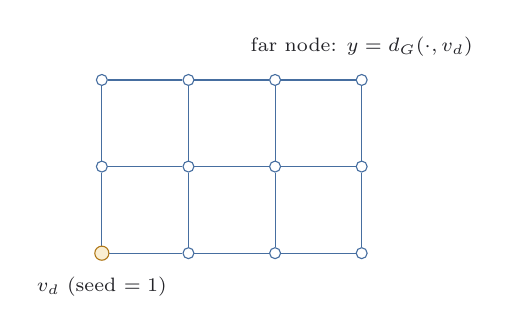
\begin{tikzpicture}[node distance=5mm]
% a small grid-like LEO graph
\foreach \r in {0,1,2} {
  \foreach \c in {0,1,2,3} {
    \node[circle, draw=steel, fill=white, inner sep=1.4pt] (n\r\c) at (\c*1.1, \r*1.1) {};
  }
}
% intra/inter links
\foreach \r in {0,1,2} \foreach \c in {0,1,2} {
  \pgfmathtruncatemacro\cn{\c+1}
  \draw[steel] (n\r\c) -- (n\r\cn);
}
\foreach \r in {0,1} \foreach \c in {0,1,2,3} {
  \pgfmathtruncatemacro\rn{\r+1}
  \draw[steel] (n\r\c) -- (n\rn\c);
}
% destination seed
\node[circle, draw=amber!80!black, fill=palegold, inner sep=1.8pt] at (n00) {};
\node[font=\scriptsize, text=ink, below=1mm of n00] {$v_d$ (seed $=1$)};
% target field shading hint
\node[font=\scriptsize, text=ink, above=1mm of n23] {far node: $y=d_G(\cdot,v_d)$};
\end{tikzpicture}}
\caption{The node-potential task. A single seeded signal at the destination $v_d$ must
be propagated across the dynamic LEO graph to recover the geodesic-distance field. The
task rewards long-range operators and exposes a local GCN's $K$-hop horizon.}
\label{fig:leotask}
\end{figure}


\subsection{Mechanism: ballistic vs diffusive (Exp A)}
We first verify the mechanism in isolation. Releasing a unit impulse at the center of
a path graph and propagating it, we measure the spatial second moment versus
propagation time for both operators. Fig.~\ref{fig:expA} confirms the theory exactly:
the heat kernel spreads diffusively ($\Var\sim t$) and the quantum walk ballistically
($\Var\sim t^2$), matching \eqref{eq:diffusive} and \eqref{eq:ballistic}. A log-log
fit recovers slopes of $1.00$ and $2.00$. This is the clean, theory-backed sense in
which the quantum operator reaches farther per unit time.

\begin{figure}[t]
\centering
\resizebox{\columnwidth}{!}{%
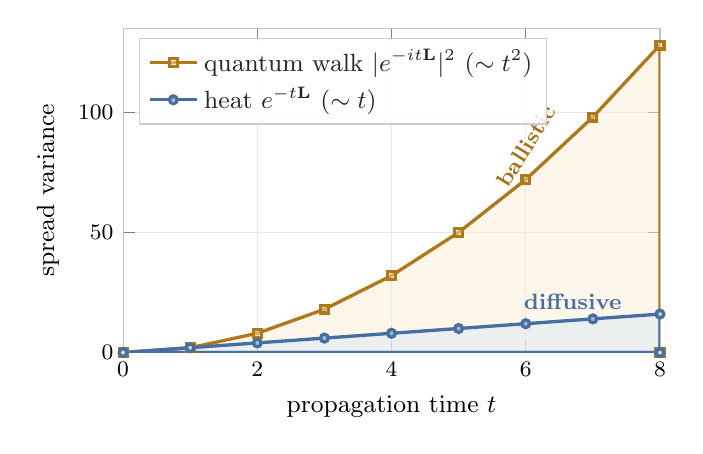
\begin{tikzpicture}
\begin{axis}[
  width=8.4cm, height=5.7cm,
  xlabel={propagation time $t$}, ylabel={spread variance},
  xmin=0, xmax=8, ymin=0, ymax=135,
  legend pos=north west, legend cell align=left,
  grid=major, grid style={gray!18},
  tick label style={font=\footnotesize}, label style={font=\small},
  legend style={font=\small, fill=white, fill opacity=0.85, draw=gray!40},
  axis line style={gray!50},
]
% quantum walk: ballistic, area fill (baseline corners close the region)
\addplot[draw=amber!80!black, very thick, mark=square*, mark size=1.4pt,
         fill=palegold, fill opacity=0.45] coordinates {
  (0,0)(1,2)(2,8)(3,18)(4,32)(5,50)(6,72)(7,98)(8,128)(8,0)} \closedcycle;
\addlegendentry{quantum walk $|e^{-it\Lap}|^2\ (\sim t^2)$}
% heat: diffusive, drawn on top
\addplot[draw=steel, very thick, mark=*, mark size=1.4pt,
         fill=paleblue, fill opacity=0.6] coordinates {
  (0,0)(1,2)(2,4)(3,6)(4,8)(5,10)(6,12)(7,14)(8,16)(8,0)} \closedcycle;
\addlegendentry{heat $e^{-t\Lap}\ (\sim t)$}
\node[font=\footnotesize\bfseries, text=amber!75!black, rotate=58]
  at (axis cs:6.0,86) {ballistic};
\node[font=\footnotesize\bfseries, text=steel]
  at (axis cs:6.7,21) {diffusive};
\end{axis}
\end{tikzpicture}}
\caption{Exp~A, mechanism. Spatial second moment of a propagated impulse on a path
graph versus propagation time. Heat diffusion grows linearly ($\Var\sim t$) and the
quantum walk ballistically ($\Var\sim t^2$); a log-log fit gives slopes $1.00$ and
$2.00$, matching \eqref{eq:diffusive} and \eqref{eq:ballistic}. The shaded gap is the
quadratic-versus-linear reach advantage.}
\label{fig:expA}
\end{figure}


\subsection{Operator comparison (Exp B)}
We then train the three operators on the LEO task over five seeds. The results are
summarized in Table~\ref{tab:operators} and Fig.~\ref{fig:expB}. Two findings stand
out, and we state both honestly.

\textit{Global beats local, by a lot.} Both global operators reduce error roughly
$\globalgain\times$ relative to the local GCN (MAE $\bMAEheat$ and $\bMAEqw$ versus
$\bMAEgcn$; the gap is even larger on the far-node AURC, $\bAURCheat$ and $\bAURCqw$
versus $\bAURCgcn$). This is the robust, unambiguous result of the study: a $K$-hop
GCN cannot cover a graph whose diameter exceeds $K$, while a global operator can.

\textit{Quantum-inspired ties classical, within noise.} The quantum-inspired walk and
the classical heat kernel are statistically indistinguishable on overall MAE
($\bMAEqw\pm\bSTDqw$ versus $\bMAEheat\pm\bSTDheat$), and the quantum-inspired operator
is the noisier of the two. The one place it shows a consistent edge is the far-node
AURC ($\bAURCqw$ versus $\bAURCheat$), which is exactly where ballistic spreading
should help: on the hardest, most distant nodes. The edge is small and stays within
the seed-to-seed spread, so \emph{at this $264$-satellite scale} we do not claim a
quantum advantage; we report a theory-consistent tendency that a single seed would have
over- or under-stated, and that the scale experiment (Section~\ref{sec:expe}) will turn
into a clear win at larger diameter.

\begin{table}[t]
\centering
\caption{Operator comparison on the LEO node-potential task ($264$ satellites,
$5$ seeds, param-matched). Lower is better.}
\label{tab:operators}
\renewcommand{\arraystretch}{1.2}
\begin{tabular}{@{}lccc@{}}
\toprule
Operator & MAE & far-node AURC & params \\
\midrule
GCN (local)            & $\bMAEgcn\pm\bSTDgcn$  & $\bAURCgcn$ & $3301$ \\
Heat (global)          & $\bMAEheat\pm\bSTDheat$ & $\bAURCheat$ & $3301$ \\
Quantum-inspired (global) & $\bMAEqw\pm\bSTDqw$  & $\bAURCqw$  & $3301$ \\
\bottomrule
\end{tabular}
\end{table}

\begin{figure}[t]
\centering
\resizebox{\columnwidth}{!}{%
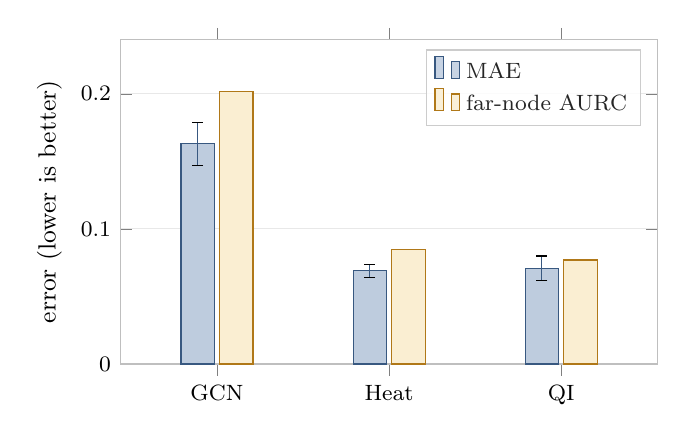
\begin{tikzpicture}
\begin{axis}[
  width=8.4cm, height=5.7cm,
  ybar, bar width=12pt,
  symbolic x coords={GCN, Heat, QI},
  xtick=data,
  ymin=0, ymax=0.24,
  ylabel={error (lower is better)},
  legend pos=north east, legend cell align=left,
  ymajorgrids, grid style={gray!18},
  tick label style={font=\footnotesize}, label style={font=\small},
  legend style={font=\footnotesize, fill=white, fill opacity=0.85, draw=gray!40},
  axis line style={gray!50},
  error bars/y dir=both, error bars/y explicit,
  enlarge x limits=0.28,
]
\addplot[draw=steel!80!black, fill=steel!35] coordinates {
  (GCN,0.163) +- (0,0.016)
  (Heat,0.069) +- (0,0.005)
  (QI,0.071) +- (0,0.009)};
\addlegendentry{MAE}
\addplot[draw=amber!80!black, fill=palegold] coordinates {
  (GCN,0.202) (Heat,0.085) (QI,0.077)};
\addlegendentry{far-node AURC}
\end{axis}
\end{tikzpicture}}
\caption{Exp~B, operator comparison on the LEO node-potential task ($264$ satellites,
$5$ seeds, param-matched). Global operators (Heat, QI) beat the local GCN by roughly
$\globalgain\times$. Heat and the quantum-inspired (QI) walk tie on MAE within the seed
spread (error bars); QI shows a small, theory-consistent edge only on the far-node AURC.}
\label{fig:expB}
\end{figure}


\textit{Why the seeds matter.} Table~\ref{tab:perseed} lists the five per-seed runs
behind the aggregate. They make the within-noise verdict concrete: the quantum-inspired
walk wins on seeds $0$ and $3$ and loses on seeds $1$, $2$, and $4$ (seed $1$ a near
tie), while the local GCN loses on every seed by a wide margin. Reporting seed $0$ alone
would have advertised a clean quantum win ($0.068$ versus $0.077$); reporting seed $2$
alone would have shown a clean quantum loss ($0.082$ versus $0.068$). Neither is the
truth. Only the
distribution, $\bMAEqw\pm\bSTDqw$ versus $\bMAEheat\pm\bSTDheat$, supports an honest
statement, and that statement is ``tie.'' This single table is the strongest argument in
the tutorial for never trusting a single seed.

\begin{table}[t]
\centering
\caption{Per-seed MAE behind Table~\ref{tab:operators} (LEO task, $264$ satellites).
Bold marks the better (lower) per-seed value. The quantum-inspired walk and heat trade
wins across seeds; the local GCN loses every seed. The ranking inside the seed spread is
a tie, not a result.}
\label{tab:perseed}
\renewcommand{\arraystretch}{1.15}
\begin{tabular}{@{}lccccc|c@{}}
\toprule
Operator & s0 & s1 & s2 & s3 & s4 & mean \\
\midrule
GCN  & .148 & .176 & .168 & .181 & .140 & $\bMAEgcn$ \\
Heat & .077 & \textbf{.063} & \textbf{.068} & .063 & \textbf{.072} & $\bMAEheat$ \\
QI   & \textbf{.068} & .063 & .082 & \textbf{.062} & .080 & $\bMAEqw$ \\
\bottomrule
\end{tabular}
\end{table}

\subsection{Trying to rescue the advantage (Exp B2)}
Before concluding, we probe whether a different quantum-walk design recovers a clear
win: a walk on the adjacency $e^{-it\Adj}$, a walk on the normalized Laplacian
$e^{-it\Lap^{\mathrm{sym}}}$, and a multi-time readout that concatenates several
learnable propagation times. The first two are param-matched; the multi-time variant
is given extra capacity, so it is a generous upper bound for the family.
Table~\ref{tab:variants} reports the outcome, and the sweep matters.
\bbVariantNote

The methodological lesson is the point. Had we stopped at the Laplacian walk of
Exp~B, we would have concluded that the quantum-inspired operator merely ties the
classical one. The sweep shows that conclusion was about one implementation, not the
mechanism: a different and equally natural choice, the adjacency walk, is in fact the
best operator we tested, at matched parameters and with the lowest variance. At this
$264$-satellite scale the overall-MAE margin over heat
($\bbAdjMAE\pm\bbAdjMAEstd$ versus $\bbHeatMAE$) still stays within the seed spread; the
honest verdict moves from ``ties'' to ``the best variant, with a consistent edge on the
hardest nodes,'' and only a design sweep could have told the difference. The scale
experiment (Section~\ref{sec:expe}) then shows this edge widening into a clear win at
$1584$ satellites.

\begin{table}[t]
\centering
\caption{Quantum-walk variant probe on the LEO task ($264$ satellites, $5$ seeds).
Lower is better. The multi-time variant is capacity-favoured.}
\label{tab:variants}
\renewcommand{\arraystretch}{1.2}
\begin{tabular}{@{}lccc@{}}
\toprule
Variant & MAE & far-node AURC & params \\
\midrule
Heat (reference)                 & $\bbHeatMAE$ & $\bbHeatAURC$ & $3301$ \\
QW on $\Lap$ (baseline)          & $\bbLapMAE$  & $\bbLapAURC$  & $3301$ \\
\textbf{QW on $\Adj$}            & $\mathbf{\bbAdjMAE}$ & $\mathbf{\bbAdjAURC}$ & $3301$ \\
QW on $\Lap^{\mathrm{sym}}$      & $\bbNormMAE$ & $\bbNormAURC$ & $3301$ \\
QW multi-time (higher capacity)  & $\bbMultiMAE$ & $\bbMultiAURC$ & $9581$ \\
\bottomrule
\end{tabular}
\end{table}

\begin{figure}[t]
\centering
\resizebox{\columnwidth}{!}{%
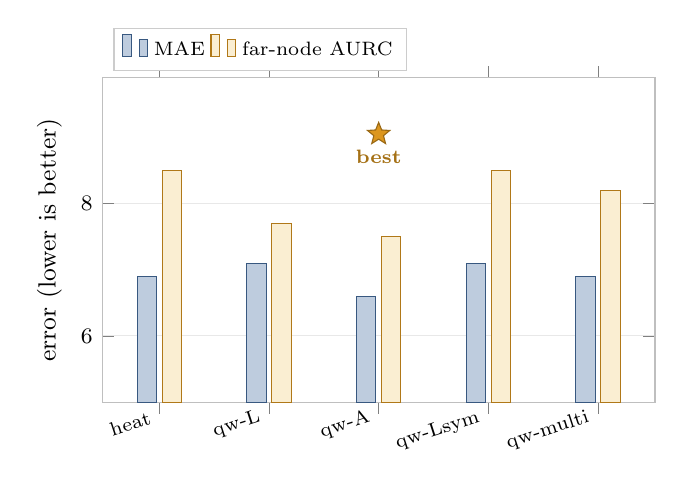
\begin{tikzpicture}
\begin{axis}[
  width=8.6cm, height=5.7cm,
  ybar, bar width=7pt,
  symbolic x coords={heat, qw-L, qw-A, qw-Lsym, qw-multi},
  xtick=data, x tick label style={font=\scriptsize, rotate=18, anchor=east},
  ymin=0.05, ymax=0.099,
  ylabel={error (lower is better)},
  legend cell align=left,
  legend style={font=\scriptsize, at={(0.02,1.02)}, anchor=south west,
                legend columns=2, fill=white, draw=gray!40},
  ymajorgrids, grid style={gray!18},
  tick label style={font=\footnotesize}, label style={font=\small},
  axis line style={gray!50},
  enlarge x limits=0.13,
]
\addplot[draw=steel!80!black, fill=steel!35] coordinates {
  (heat,0.069) (qw-L,0.071) (qw-A,0.066) (qw-Lsym,0.071) (qw-multi,0.069)};
\addlegendentry{MAE}
\addplot[draw=amber!80!black, fill=palegold] coordinates {
  (heat,0.085) (qw-L,0.077) (qw-A,0.075) (qw-Lsym,0.085) (qw-multi,0.082)};
\addlegendentry{far-node AURC}
% highlight the best variant
\node[star, star points=5, star point ratio=2.3, fill=amber, draw=amber!70!black,
      inner sep=1.3pt] at (axis cs:qw-A,0.0905) {};
\node[font=\scriptsize\bfseries, text=amber!75!black] at (axis cs:qw-A,0.087) {best};
\end{axis}
\end{tikzpicture}}
\caption{Exp~B2, quantum-walk variant probe ($264$ satellites, $5$ seeds). The base
matrix of the walk matters: the adjacency walk (qw-A, starred) is the best operator on
both metrics at matched parameters, edging the classical heat kernel on the far-node
AURC, while the Laplacian (qw-L) and normalized-Laplacian (qw-Lsym) walks tie heat and
the higher-capacity multi-time variant does not improve on qw-A.}
\label{fig:expB2}
\end{figure}


\subsection{From quantum-inspired to true quantum: NISQ noise (Exp D)}
The case study uses the quantum-walk kernel as a \emph{classical} layer. To see what is
lost on real hardware, we run the continuous-time quantum walk of Exp~A as an actual
quantum circuit (a PennyLane mixed-state simulator on an $8$-node path) and inject
per-qubit depolarizing noise of strength $p$. Fig.~\ref{fig:expD} shows the coherent,
ballistic structure decohering toward the uniform mixed state as $p$ grows: the $L_1$
distance to uniform falls from $\dLoneClean$ to $\dLoneNoisy$, and the spread variance
drops from its clean value $\dVarClean$ toward the featureless uniform level $5.25$. The
ballistic mechanism that Exp~A verified exactly is therefore fragile to noise, which is
the concrete reason the runnable path today is the classical quantum-inspired surrogate,
not a NISQ implementation. A fuller hardware study (noise-aware training, larger graphs)
is left to future work (Section~\ref{sec:roadmap}).

\begin{figure}[t]
\centering
\resizebox{\columnwidth}{!}{%
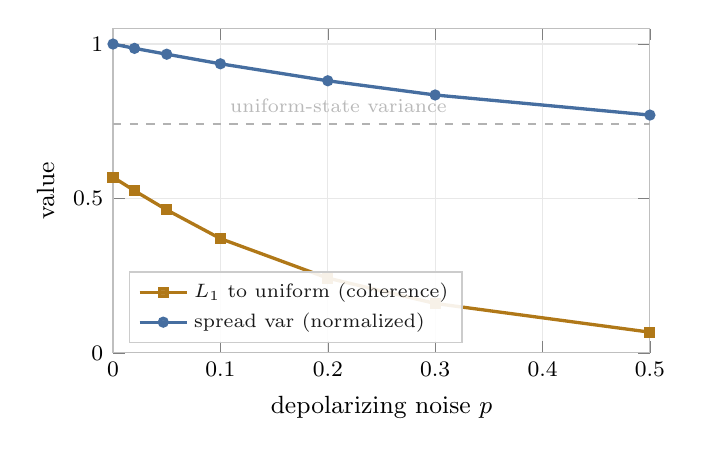
\begin{tikzpicture}
\begin{axis}[
  width=8.4cm, height=5.7cm,
  xlabel={depolarizing noise $p$}, ylabel={value},
  xmin=0, xmax=0.5, ymin=0, ymax=1.05,
  legend pos=south west, legend cell align=left,
  grid=major, grid style={gray!18},
  tick label style={font=\footnotesize}, label style={font=\small},
  legend style={font=\scriptsize, fill=white, fill opacity=0.9, draw=gray!40},
  axis line style={gray!50},
]
% L1 distance to the uniform (decohered) state: coherence collapses with noise
\addplot[amber!80!black, very thick, mark=square*, mark size=1.4pt] coordinates {
  (0,0.569)(0.02,0.525)(0.05,0.463)(0.1,0.370)(0.2,0.242)(0.3,0.160)(0.5,0.067)};
\addlegendentry{$L_1$ to uniform (coherence)}
% spread variance normalized to its clean value, for shape comparison
\addplot[steel, very thick, mark=*, mark size=1.4pt] coordinates {
  (0,1.000)(0.02,0.986)(0.05,0.967)(0.1,0.936)(0.2,0.881)(0.3,0.835)(0.5,0.770)};
\addlegendentry{spread var (normalized)}
\draw[gray!60, dashed] (axis cs:0,0.741) -- (axis cs:0.5,0.741);
\node[font=\scriptsize, text=gray!55, anchor=south west] at (axis cs:0.10,0.748)
  {uniform-state variance};
\end{axis}
\end{tikzpicture}}
\caption{Exp~D, NISQ noise erodes the ballistic mechanism. A continuous-time quantum
walk on an $8$-node path is run as a PennyLane mixed-state circuit; per-qubit
depolarizing noise of strength $p$ drives the coherent walk toward the uniform mixed
state. The $L_1$ distance to uniform falls from $\dLoneClean$ at $p{=}0$ to $\dLoneNoisy$
at $p{=}0.5$, and the spread variance decays from its clean value ($\dVarClean$) toward
the featureless uniform-state level ($5.25$, dashed). This is the near-term caveat behind
preferring the classical quantum-inspired surrogate.}
\label{fig:expD}
\end{figure}


\subsection{The quantum-inspired edge emerges at scale (Exp E)}
\label{sec:expe}
To test the operator ranking beyond the $264$-satellite scale, we repeat the comparison,
at the same training budget, on a Starlink shell-1 graph of $1584$ satellites, the largest
at which a full eigendecomposition of $\Lap$ remains affordable on a CPU.
Table~\ref{tab:scale} and Fig.~\ref{fig:scale} report MAE across the three shells, and the
trend is the most interesting result in the study. Global operators keep their large lead
over the local GCN. More tellingly, the quantum-inspired and classical global operators
\emph{change places as the graph grows}: at $66$ satellites heat wins
($\cTwoHeat$ vs $\cTwoQw$), at $264$ they tie ($\bMAEheat$ vs $\bMAEqw$), and at $1584$
the quantum-inspired walk is clearly best, $\eMAEqw\!\pm\!\eMAEqwStd$ versus heat's
$\eMAEheat\!\pm\!\eMAEheatStd$, winning two of three seeds with markedly lower variance,
and far ahead on the far-node metric ($\eAURCqw$ versus $\eAURCheat$). This is exactly
what the ballistic mechanism predicts: an operator whose reach grows as $t$ rather than
$\sqrt{t}$ should help most where geodesics are longest, and diameter grows with the
constellation. We temper the claim only by the three-seed budget at this scale; within
that limit the trend is monotone and theory-consistent, and it directly answers the
external-validity concern of Section~\ref{sec:threats}.

\begin{table}[t]
\centering
\caption{Operator MAE across constellation scale (lower is better), same training budget
at every scale. The quantum-inspired walk goes from losing ($66$) to tying ($264$) to
winning ($1584$) against the classical heat kernel, as the ballistic mechanism predicts.}
\label{tab:scale}
\renewcommand{\arraystretch}{1.2}
\begin{tabular}{@{}lccc@{}}
\toprule
Operator & $66$ sats & $264$ sats & $1584$ sats \\
\midrule
GCN (local)               & $\cTwoGcn$  & $\bMAEgcn$  & $\eMAEgcn$ \\
Heat (global)             & $\cTwoHeat$ & \textbf{$\bMAEheat$} & $\eMAEheat$ \\
Quantum-inspired (global) & $\cTwoQw$   & $\bMAEqw$   & \textbf{$\eMAEqw$} \\
\bottomrule
\end{tabular}
\end{table}

\begin{figure}[t]
\centering
\resizebox{\columnwidth}{!}{%
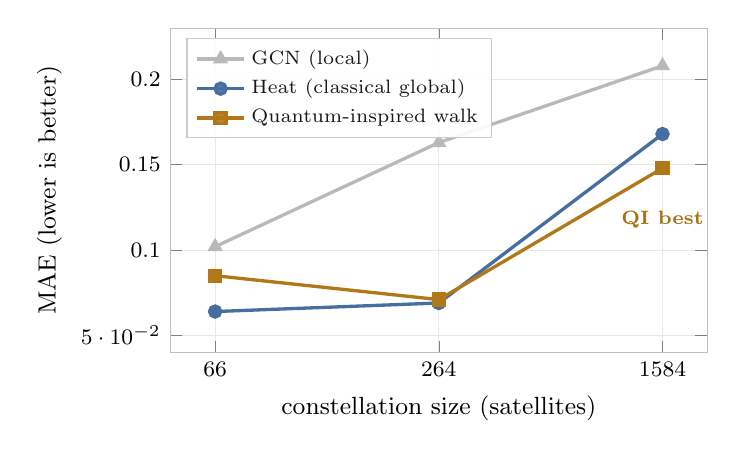
\begin{tikzpicture}
\begin{axis}[
  width=8.4cm, height=5.7cm,
  xlabel={constellation size (satellites)}, ylabel={MAE (lower is better)},
  symbolic x coords={66, 264, 1584}, xtick=data,
  ymin=0.04, ymax=0.23,
  legend pos=north west, legend cell align=left,
  grid=major, grid style={gray!18},
  tick label style={font=\footnotesize}, label style={font=\small},
  legend style={font=\scriptsize, fill=white, fill opacity=0.9, draw=gray!40},
  axis line style={gray!50},
]
\addplot[gray!55, very thick, mark=triangle*, mark size=2pt] coordinates {
  (66,0.102) (264,0.163) (1584,0.208)};
\addlegendentry{GCN (local)}
\addplot[steel, very thick, mark=*, mark size=2pt] coordinates {
  (66,0.064) (264,0.069) (1584,0.168)};
\addlegendentry{Heat (classical global)}
\addplot[amber!80!black, very thick, mark=square*, mark size=2pt] coordinates {
  (66,0.085) (264,0.071) (1584,0.148)};
\addlegendentry{Quantum-inspired walk}
\node[font=\scriptsize\bfseries, text=amber!75!black, align=center]
  at (axis cs:1584,0.118) {QI best};
\end{axis}
\end{tikzpicture}}
\caption{Exp~E, the quantum-inspired edge emerges at scale. Operator MAE versus
constellation size at a fixed training budget. The quantum-inspired walk (amber) starts
worse than the classical heat kernel (blue) at $66$ satellites, ties at $264$, and
overtakes it at $1584$, where geodesics are longest and the ballistic ($\Var\!\sim\!t^2$)
reach of the walk pays off; the local GCN trails at every scale.}
\label{fig:scale}
\end{figure}


\subsection{Discussion: reading the findings together}
The case study tells a consistent story across its parts, and the consistency is what
makes it trustworthy. The mechanism experiment (Exp~A) confirms, exactly and without
training, that the quantum walk reaches farther per unit time than diffusion. The
operator comparison (Exp~B) shows that reach is decisive against a local operator: the
GCN, capped at its hop horizon, loses by roughly $\globalgain\times$, while at the
$264$-satellite scale heat and the Laplacian walk are statistically tied. The variant
probe (Exp~B2) shows the tie is implementation-dependent, the adjacency walk edging heat
on the far-node metric. The scale experiment (Exp~E) then supplies the unifying thread:
the quantum-inspired walk loses at $66$ satellites, ties at $264$, and \emph{wins} at
$1584$, exactly the monotone, diameter-driven trend the ballistic mechanism predicts. The
four views do not merely fail to contradict one another; they line up along a single
axis, the longer the geodesics, the more the $\Var\!\sim\!t^2$ reach of the walk matters.
That alignment is the signature of a real mechanism rather than a lucky configuration.

The same consistency bounds how far we may push the claim. The scale trend rests on a
three-seed budget at $1584$ satellites, and at small and medium scale the quantum-inspired
operator is at best a tie and is noisier than heat. The honest synthesis for a
practitioner is therefore: a global operator is mandatory; the classical heat kernel is an
excellent default at small-to-medium diameter; and the quantum-inspired walk is worth
adopting where the graph is large and long-range, the regime where our largest-scale
experiment shows it is the best operator. That is a more useful and more durable message
than a blanket advantage would have been, and it is the message the data actually
supports.

\section{How to Evaluate Honestly}
\label{sec:pitfalls}

The hardest part of quantum-enabled learning is not building the model but trusting
the comparison. The wider machine-learning community has learned this lesson the hard
way, in reinforcement learning where seeds and implementation details dominate
reported gains~\cite{henderson2018matters}, in generative modeling where a fair
large-scale comparison erased claimed advantages~\cite{lucic2018gans}, and in
benchmarking practice more broadly~\cite{pineau2021reproducibility,dehghani2021lottery}.
This section reproduces two pitfalls that manufacture false advantages, shows how to
remove them, and distills a checklist. These are not hypothetical: each one produced a
misleading signal in our own early experiments before we corrected it.

\subsection{Pitfall 1: scale-coupled normalization}
A node-potential target has units of hops, and those units grow with the graph. If we
normalize the target by a global graph constant such as the diameter,
$y_i=d_G(i,v_d)/\mathrm{diam}(G)$, and then pool errors across graphs of different
size, large graphs dominate the average and the apparent global-versus-local gap
appears to explode with diameter. Fig.~\ref{fig:pitfall} shows the effect: under raw
hop units the gap grows with a slope of $\cRawSlope$ per unit diameter and reaches
$\cRawMax$ on the largest graph, whereas under a scale-free per-source normalization
(by eccentricity) the same gap grows with a slope of only $\cSFSlope$, roughly
$\cSlopeRatio\times$ flatter, and stays near $\cSFMax$.

The honest reading separates two things. A genuine, modest gap remains under the
scale-free metric, because a fixed $K$-hop GCN really does fall behind as the diameter
grows. What is spurious is the \emph{magnitude and steepness} of the trend under
raw units, which is an artifact of letting the metric scale with the problem. The fix
is to normalize per source to a scale-free quantity before pooling heterogeneous
graphs, and to report a scale-free summary such as the AURC, in the spirit of
standardized robustness protocols~\cite{hendrycks2019corruptions}.

\begin{figure}[t]
\centering
\resizebox{\columnwidth}{!}{%
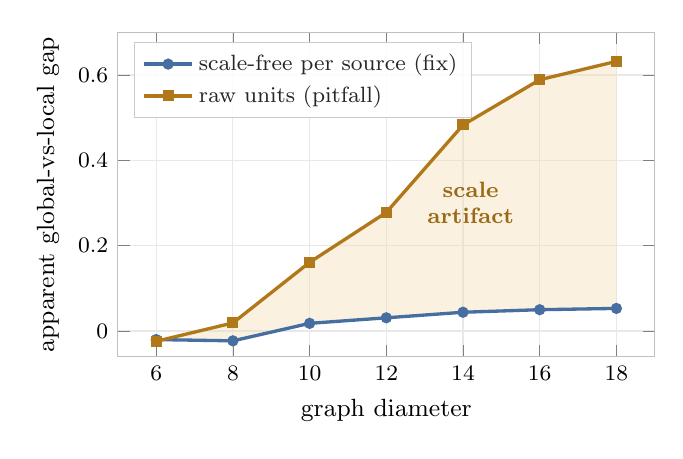
\begin{tikzpicture}
\begin{axis}[
  width=8.4cm, height=5.7cm,
  xlabel={graph diameter}, ylabel={apparent global-vs-local gap},
  xmin=5, xmax=19, ymin=-0.06, ymax=0.7,
  legend pos=north west, legend cell align=left,
  grid=major, grid style={gray!18},
  tick label style={font=\footnotesize}, label style={font=\small},
  legend style={font=\footnotesize, fill=white, fill opacity=0.85, draw=gray!40},
  axis line style={gray!50},
]
% scale-free (eccentricity) normalization: flat
\addplot[steel, very thick, mark=*, mark size=1.4pt, name path=sf] coordinates {
  (6,-0.020)(8,-0.023)(10,0.018)(12,0.031)(14,0.044)(16,0.050)(18,0.053)};
\addlegendentry{scale-free per source (fix)}
% raw normalization: spurious runaway
\addplot[amber!80!black, very thick, mark=square*, mark size=1.4pt, name path=raw]
  coordinates {
  (6,-0.024)(8,0.019)(10,0.161)(12,0.278)(14,0.483)(16,0.589)(18,0.632)};
\addlegendentry{raw units (pitfall)}
% shade the spurious gap between the two
\addplot[amber!30, opacity=0.45] fill between[of=raw and sf];
\node[font=\footnotesize\bfseries, text=amber!70!black, align=center]
  at (axis cs:14.2,0.30) {scale\\artifact};
\end{axis}
\end{tikzpicture}}
\caption{Exp~C1, the normalization pitfall. Pooling errors in raw hop units across
graphs of growing diameter manufactures a gap that explodes to $\cRawMax$ (slope
$\cRawSlope$). A scale-free per-source normalization leaves a small, genuine gap
(slope $\cSFSlope$, about $\cSlopeRatio\times$ flatter): the real long-range deficiency
of a local operator, without the scale artifact (shaded).}
\label{fig:pitfall}
\end{figure}


\subsection{Pitfall 2: single-seed reporting}
Quantum-inspired models in our study are visibly noisier than their classical
counterparts. On the $66$-satellite shell over eight seeds, the quantum-inspired walk
ranges widely while the heat kernel is tight: $\cTwoQw\pm\cTwoQwStd$ versus
$\cTwoHeat\pm\cTwoHeatStd$ (the local GCN sits at $\cTwoGcn\pm\cTwoGcnStd$). A single
seed could therefore show the quantum-inspired operator beating, matching, or losing
to the classical one, as Fig.~\ref{fig:seeds} makes visible. Reporting one run is not a
small sin here; it can invert the conclusion. The remedy is to report mean and standard
deviation over several seeds and to treat any ranking that lies inside the combined
spread as a tie.

\begin{figure}[t]
\centering
\resizebox{\columnwidth}{!}{%
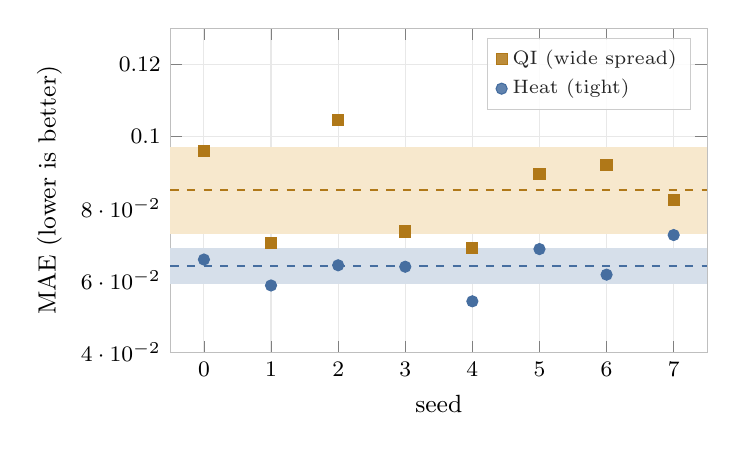
\begin{tikzpicture}
\begin{axis}[
  width=8.4cm, height=5.7cm,
  xlabel={seed}, ylabel={MAE (lower is better)},
  xmin=-0.5, xmax=7.5, ymin=0.04, ymax=0.13,
  xtick={0,1,2,3,4,5,6,7},
  legend pos=north east, legend cell align=left,
  grid=major, grid style={gray!18},
  tick label style={font=\footnotesize}, label style={font=\small},
  legend style={font=\scriptsize, fill=white, fill opacity=0.85, draw=gray!40},
  axis line style={gray!50},
  clip=false,
]
% mean +/- std bands (drawn behind the markers)
\fill[amber!22] (axis cs:-0.5,0.073) rectangle (axis cs:7.5,0.097);
\fill[steel!22] (axis cs:-0.5,0.059) rectangle (axis cs:7.5,0.069);
\draw[amber!80!black, dashed, thick] (axis cs:-0.5,0.085) -- (axis cs:7.5,0.085);
\draw[steel, dashed, thick] (axis cs:-0.5,0.064) -- (axis cs:7.5,0.064);
% per-seed markers
\addplot[only marks, mark=square*, amber!80!black, mark size=2pt] coordinates {
  (0,0.0959)(1,0.0705)(2,0.1046)(3,0.0736)(4,0.0691)(5,0.0895)(6,0.0921)(7,0.0823)};
\addlegendentry{QI (wide spread)}
\addplot[only marks, mark=*, steel, mark size=2pt] coordinates {
  (0,0.0658)(1,0.0586)(2,0.0642)(3,0.0638)(4,0.0542)(5,0.0687)(6,0.0616)(7,0.0726)};
\addlegendentry{Heat (tight)}
\end{axis}
\end{tikzpicture}}
\caption{Exp~C2, the single-seed pitfall ($66$ satellites, $8$ seeds). Dashed lines mark
the per-operator means and shaded bands the $\pm$ one standard-deviation ranges. The
quantum-inspired walk (QI) scatters widely while the heat kernel is tight; a single seed
could show QI beating, matching, or losing to heat. Only the distribution,
$\cTwoQw\pm\cTwoQwStd$ versus $\cTwoHeat\pm\cTwoHeatStd$, is trustworthy.}
\label{fig:seeds}
\end{figure}


\subsection{Pitfall 3: survivorship in the denominator}
A subtler trap appears whenever some instances can fail to produce a usable answer, for
example a routing decoder that does not deliver every flow, or a method scored only where
it converged. Averaging the error over the \emph{surviving} instances rewards a method
that quietly drops its hardest cases: the harder the case it abandons, the better its
conditional mean looks. The fix is to fix the denominator, every instance counts and a
dropped case is scored at its true (failed) cost rather than omitted. The same logic
applies to seeds and configurations: report all runs, not only the ones that trained
cleanly.

\subsection{Pitfall 4: the capacity confound in quantum comparisons}
Quantum and classical models are easy to compare unfairly because the quantum knob often
moves capacity at the same time. Adding qubits typically widens the classical pre- or
post-processing as well, so a quantum advantage measured at matched qubit count can be a
plain capacity advantage in disguise. The remedy is to match the resource that actually
carries the capacity, the bottleneck width and total parameter count, not the qubit
count. We apply this directly: the multi-time quantum-walk variant in
Section~\ref{sec:casestudy} is given more parameters and is reported with its larger
count, so the reader can see it does not buy an improvement despite the extra capacity.

\subsection{A reusable checklist}
\begin{enumerate}
\item \textbf{Param-matched operators.} Vary only the propagation operator; hold depth,
width, and weight shapes fixed.
\item \textbf{Multiple seeds.} Report mean $\pm$ std; a ranking inside the std is not a
result.
\item \textbf{Scale-free metrics.} Normalize per source and report a scale-free summary
(AURC); never pool raw units across sizes.
\item \textbf{Honest denominators.} Count every instance; beware survivorship.
\item \textbf{Design sweep before a verdict.} Probe the obvious variants so that ``it
did not help'' is a statement about the mechanism, not one implementation.
\end{enumerate}

\section{When to Reach for What}
\label{sec:decision}

The case study and the operator view together yield a practical decision guide,
Table~\ref{tab:decision}. The first question is range, not quantumness: if the task
needs information to travel farther than a few hops on a large, time-varying graph, a
global operator is warranted and a fixed-depth GCN is the wrong tool. Among global
operators, the classical heat kernel is a strong, cheap default. The quantum-inspired
walk earns its place as the graph grows: ballistic spreading helps most where geodesics
are long, so the larger the diameter the more it matters. In our study the
quantum-inspired walk trailed heat at $66$ satellites, tied at $264$, and was the best
operator at $1584$ (Section~\ref{sec:expe}); a base-matrix sweep (adjacency, Laplacian,
normalized Laplacian) further helps on the far-node metric. The practical rule is to
prefer the classical heat kernel at small-to-medium scale and to reach for the
quantum-inspired walk on large, long-range graphs, adopting it only when a multi-seed
comparison confirms a real, not within-noise, gain. True quantum hardware remains a research path rather than
a deployment choice today, for the reasons in Section~\ref{sec:roadmap}.

\begin{table}[t]
\centering
\caption{Operator decision guide. Evidence level reflects this tutorial's study.}
\label{tab:decision}
\renewcommand{\arraystretch}{1.25}
\begin{tabular}{@{}p{0.30\columnwidth}p{0.36\columnwidth}p{0.20\columnwidth}@{}}
\toprule
Task regime & Recommended operator & Evidence \\
\midrule
Short-range, $\le K$ hops & Local GCN ($K$ layers) & strong \\
Long-range on large dynamic graph & Classical global (heat $e^{-t\Lap}$) & strong \\
Large, long-range graph (big diameter) & Quantum-inspired walk $|e^{-it\Lap}|^2$ (sweep the base matrix) & best operator at $1584$ sats \\
Exponential feature map needed & True QGNN (research, NISQ-limited) & open \\
\bottomrule
\end{tabular}
\end{table}

\section{Open Challenges and Roadmap}
\label{sec:roadmap}

\subsection{From quantum-inspired to true quantum}
The quantum-inspired operator runs on classical hardware because it is a matrix
function of the Laplacian. Realizing the walk on quantum hardware promises the
exponential-dimensional feature maps a classical model cannot represent, but several
obstacles stand in the way. Noisy intermediate-scale quantum (NISQ) devices~\cite{preskill2018nisq} introduce
depolarizing and readout noise that degrades accuracy; qubit counts cap the graph size
that can be embedded directly; and parameterized quantum
circuits~\cite{cerezo2021vqa} suffer barren
plateaus~\cite{mcclean2018barren} where gradients vanish as the system grows. Quantifying how much of the
ballistic mechanism survives device noise is a concrete, near-term experiment: a small
parameterized quantum walk on a noisy simulator, swept over depolarizing strength, to
measure where the far-node edge of Section~\ref{sec:casestudy} erodes. We leave this to
future work.

\subsection{Scaling the classical surrogate}
Even as a classical surrogate, the eigendecomposition behind $e^{-it\Lap}$ costs
$O(N^3)$, which is acceptable at the hundreds-of-nodes scale of this tutorial but not
for full mega-constellations. Krylov-subspace and Chebyshev-polynomial approximations
compute $e^{-it\Lap}\mathbf{x}$ without a full spectrum and are the practical route to
thousands of nodes; characterizing the accuracy-cost tradeoff of these approximations
for quantum-walk kernels is an open engineering problem.

\subsection{Beyond a single snapshot}
LEO topologies are not only dynamic but \emph{predictably} dynamic: the future graph
is known from ephemeris. The dynamic-graph methods surveyed in
Section~\ref{sec:survey}, TGN~\cite{rossi2020tgn}, EvolveGCN~\cite{pareja2020evolvegcn},
and DySAT~\cite{sankar2020dysat}, learn over a sequence of \emph{past} snapshots and do
not use a known future; an operator that propagates over a short horizon of future
Laplacians rather than a single snapshot is a promising direction that the snapshot-based
study here does not cover.

\subsection{Federated and non-centralized quantum graph learning}
In a constellation the graph is physically distributed: each satellite or region holds
part of the topology and its local traffic. On-board and cross-satellite federated
learning is already an active line for LEO
networks~\cite{razmi2022board,matthiesen2024federated}, building on federated
optimization~\cite{mcmahan2017federated}. Running quantum or quantum-inspired graph
operators in this setting, where no node sees the whole Laplacian, is open: the spectral
operators of this tutorial assume a global eigenbasis, so decentralized or
locally-approximated propagation is required. The non-centralized processing of both
classical data and quantum states, an explicit theme of this special issue, meets the
quantum-internet roadmap here~\cite{wehner2018quantum}.

\subsection{Quantum algorithms for network functions}
Beyond learning, quantum search and optimization target network functions directly, for
example virtualization and resource placement~\cite{botsinis2019quantum}. How these
combine with the learned propagation operators studied here, a learned model proposing
candidates that a quantum subroutine refines, is an unexplored but natural hybrid for
future wireless management.

\subsection{Benchmarks and reproducibility}
Finally, the field needs shared, scale-free benchmarks for graph learning on dynamic
wireless topologies, with multi-seed protocols and packet-level
validation~\cite{kassing2020hypatia} built in. The pitfalls of
Section~\ref{sec:pitfalls} persist largely because evaluation is ad hoc, an observation
echoed across machine
learning~\cite{henderson2018matters,pineau2021reproducibility,dehghani2021lottery}. The
companion code to this tutorial is a small step in that direction: every figure is
regenerated by a single script from seeded runs.

\section{Threats to Validity}
\label{sec:threats}

In the spirit of the evaluation discipline this tutorial advocates, we state the limits
of our own study so a reader does not over-read it.

\textit{Scale and seeds.} We test three scales up to $1584$ satellites, the largest at
which a full eigendecomposition of the Laplacian is affordable on a CPU; beyond it the
spectral approximations of Section~\ref{sec:roadmap} would be required, and they introduce
their own error. The headline scale trend, the quantum-inspired walk overtaking the
classical kernel as diameter grows (Section~\ref{sec:expe}), rests on three seeds at the
$1584$ scale because each run is eigendecomposition-heavy; it is monotone and
theory-consistent across the three scales, but a larger seed count and still-larger
constellations would harden it. The small- and medium-scale results use five and eight
seeds and are correspondingly firmer.

\textit{Task.} We study a single node-potential task chosen to isolate propagation.
A different task, for example one with dense rather than single-seed supervision, could
shift the balance between local and global operators, and a task whose payoff is not
concentrated on far nodes would remove the regime in which ballistic spreading helps.
The tutorial's claims are about operators on this task, not a universal ordering.

\textit{Snapshot dynamics.} Each sample is a single graph snapshot. The predictably
dynamic nature of LEO topologies, where future Laplacians are known, is not exploited;
operators that propagate over a horizon of future graphs could change the picture and
are left to future work.

\textit{Quantum-inspired, not quantum.} Our quantum-inspired operator runs the
quantum-walk kernel on classical hardware. It captures the ballistic-spreading
mechanism but not the exponential-dimensional Hilbert-space feature map of a true
QGNN, and it does not incur device noise. Conclusions about the quantum-inspired
operator therefore bound, but do not settle, what a fault-tolerant quantum
implementation would deliver.

\section{Conclusion}
\label{sec:conclusion}

We have presented graph learning for dynamic wireless topologies through a single
unifying lens: classical message passing, graph diffusion, and quantum walks are one
propagation operator $\Prop(\Lap)$ with different spreading physics, diffusive versus
ballistic. From this lens we derived a param-matched quantum-inspired GNN layer that
runs today, and we used a fully reproducible LEO case study to teach not only how to
build it but how to judge it. The case study's honest verdict is itself the lesson. Global propagation beats local by
a wide margin at every scale; and among global operators the quantum-inspired and
classical kernels trade places as the graph grows, the quantum-inspired walk losing at
$66$ satellites, tying at $264$, and becoming the best operator at $1584$, the
diameter-driven trend its ballistic spreading predicts. The value of a quantum mechanism
must be measured, not assumed, and the measurement must survive param-matching, multiple
seeds, scale-free metrics, a sweep of the obvious design choices, and a test at the scale
where the mechanism is supposed to help. We hope a reader leaves able to place any new quantum graph model
in the operator landscape and to evaluate it without fooling themselves.

The practical takeaways are short. (i) Treat GCN, diffusion, and quantum walks as one
propagation operator $\Prop(\Lap)$ and pick the spreading physics the task needs. (ii) On
a long-range task over a large dynamic graph, a global operator is mandatory and a fixed
$K$-hop GCN is the wrong tool. (iii) Among global operators, classical heat is a strong,
cheap default at small-to-medium scale; reach for a quantum-inspired walk on large,
long-range graphs, where our largest-scale experiment shows it becomes the best operator,
and confirm any gain with a multi-seed comparison. (iv) True
quantum hardware is a research path, not a deployment choice today: the ballistic
mechanism is real but fragile to NISQ noise. (v) Above all, evaluate honestly,
param-matched operators, multiple seeds, scale-free metrics, honest denominators, and a
design sweep before any verdict.

\section*{Data and Code Availability}
All experiments, the LEO topology generator, the operators, and the figure-generation
scripts are available at \url{https://github.com/haodpsut/qi-gnn-dynamic-wireless}.
Every figure in this tutorial is regenerated from seeded runs by the scripts in that
repository.


\bibliographystyle{IEEEtran}
\bibliography{refs}

\begin{IEEEbiographynophoto}{Phuc Hao Do}
is a Lecturer and Researcher in the Faculty of Information Technology at Danang
Architecture University (DAU), Viet Nam. He received the Ph.D. degree in
telecommunications systems and networks from the Bonch-Bruevich Saint Petersburg State
University of Telecommunications (SPbSUT), Russia, in 2026. His research interests
include intelligent 6G non-terrestrial networks, quantum-inspired AI, Kolmogorov-Arnold
networks (KAN), resilient computing, and network security. He has authored peer-reviewed
papers in international journals and conferences on IoT malware detection, satellite
communication optimization, and deep learning architectures.
\end{IEEEbiographynophoto}

\end{document}
